\documentclass[11pt,a4paper]{article}

% ----------------------------------------------------
% PACKAGES ESSENTIELS
% ----------------------------------------------------
\usepackage[utf8]{inputenc}        % Encodage du texte (UTF-8)
\usepackage[T1]{fontenc}           % Encodage des caractères français
\usepackage[french]{babel}         % Langue du document
\usepackage{geometry}              % Gestion des marges
\usepackage{graphicx}              % Insertion d’images
\usepackage{amsmath, amssymb}      % Symboles et équations mathématiques
\usepackage{siunitx}               % Unités du Système International (SI)
\usepackage{caption}               % Amélioration des légendes
\usepackage{subcaption}            % Sous-figures
\usepackage{booktabs}              % Tableaux esthétiques
\usepackage{float}                 % Contrôle de la position des figures
\usepackage{hyperref}              % Liens cliquables dans le PDF
\usepackage{xcolor}                % Gestion des couleurs
\usepackage{fancyhdr}              % En-têtes et pieds de page personnalisés
\usepackage{enumitem}              % Listes personnalisées
\usepackage{physics}               % Notation physique (contraintes, déformations, etc.)

% ----------------------------------------------------
% PARAMÈTRES DE MISE EN PAGE
% ----------------------------------------------------
\geometry{margin=2.5cm}            % Marges du document
\setlength{\parskip}{0.5em}        % Espacement entre les paragraphes
\setlength{\parindent}{0pt}        % Pas d’indentation au début des paragraphes

% Configuration des liens
\hypersetup{
	colorlinks=true,
	linkcolor=blue,
	urlcolor=blue,
	citecolor=gray
}

% ----------------------------------------------------
% COULEURS ENSTA
% ----------------------------------------------------
\definecolor{enstaBleuFonce}{HTML}{003366}   % Bleu marine (sections)
\definecolor{enstaBleuClair}{HTML}{0073CF}   % Bleu moyen (sous-sections)

% ----------------------------------------------------
% STYLE DES SECTIONS
% ----------------------------------------------------
\usepackage{titlesec}

% Section (bleu marine, majuscule, gras)
\titleformat{\section}
{\normalfont\huge\bfseries\color{enstaBleuFonce}}
{\thesection}{1em}{}

% Sous-section (bleu clair, gras)
\titleformat{\subsection}
{\normalfont\large\bfseries\color{enstaBleuClair}}
{\thesubsection}{1em}{}

% Sous-sous-section en noir mais plus discret
\titleformat{\subsubsection}
{\normalfont\normalsize\bfseries\color{black!70}}
{\thesubsubsection}{1em}{}

% Horizontal line
\titleformat{\section}[block]
{\normalfont\Large\bfseries\color{enstaBleuFonce}}
{\thesection}{1em}{}
[\vspace{0.3em}\titlerule\color{enstaBleuFonce}\vspace{0.3em}]


% ----------------------------------------------------
% EN-TÊTES ET PIEDS DE PAGE
% ----------------------------------------------------
\pagestyle{fancy}
\fancyhf{}
\fancyhead[L]{ENSTA Paris}
\fancyhead[R]{TP1 — Détection et Appariement de Points}
\fancyfoot[C]{\thepage}


% ----------------------------------------------------
% FANCY QUOTES
% ----------------------------------------------------
% for adjustwidth environment
\usepackage[strict]{changepage}

% for formal definitions
\usepackage{framed}

% environment derived from framed.sty: see leftbar environment definition
\definecolor{formalshade}{rgb}{0.95,0.95,1}

\newenvironment{formal}{%
	\def\FrameCommand{%
		\hspace{1pt}%
		{\color{enstaBleuFonce}\vrule width 2pt}%
		{\color{formalshade}\vrule width 4pt}%
		\colorbox{formalshade}%
	}%
	\MakeFramed{\advance\hsize-\width\FrameRestore}%
	\noindent\hspace{-4.55pt}% disable indenting first paragraph
	\begin{adjustwidth}{}{7pt}%
		\vspace{2pt}\vspace{2pt}%
	}
	{%
		\vspace{6pt}\end{adjustwidth}\endMakeFramed%
}


% ----------------------------------------------------
% PYTHON LISTING STYLE
% ----------------------------------------------------
\usepackage{listings}              % Block des codes

% Coleurs:
\usepackage[dvipsnames]{xcolor}
\definecolor{codegreen}{rgb}{0,0.6,0}
\definecolor{codegray}{rgb}{0.5,0.5,0.5}
\definecolor{codepurple}{rgb}{0.58,0,0.82}
\definecolor{backcolour}{rgb}{0.95,0.95,0.95}

\lstdefinestyle{mystyle}{
	backgroundcolor=\color{backcolour},   
	commentstyle=\color{codepurple},
	keywordstyle=\color{NavyBlue},
	numberstyle=\tiny\color{codegray},
	stringstyle=\color{codepurple},
	basicstyle=\ttfamily\footnotesize\bfseries,
	breakatwhitespace=false,         
	breaklines=true,                 
	captionpos=t,                    
	keepspaces=true,                 
	numbers=left,                    
	numbersep=5pt,                  
	showspaces=false,                
	showstringspaces=false,
	showtabs=false,                  
	tabsize=2
}

\lstset{
	style=mystyle,
	framexleftmargin=3.5mm,
	frame=shadowbox,
	rulesepcolor=\color{black},
	xleftmargin=.05\textwidth, 
	xrightmargin=.05\textwidth,
	aboveskip=12pt,
	belowskip=12pt
}

% ----------------------------------------------------
% DÉBUT DU DOCUMENT
% ----------------------------------------------------
\begin{document}
	
	% ====================================================
	% PAGE DE COUVERTURE
	% ====================================================
	\begin{titlepage}
		\centering
		
\includegraphics[width=0.6\textwidth]{logo_ensta.png}\par\vspace{1cm}
		%{\scshape\LARGE ENSTA Paris \par}
		\vspace{2cm}
		{\Large  MI204 -- Reconnaissance d’Images \par}
		\vspace{0.2cm}
		
		
		{\huge\bfseries TP1 -- Détection et Appariement de Points \par}
		\vspace{3cm}
		{\Large Maria Clara OLIVEIRA DOMINGOS RUAS \par}
		{\Large Luiz Henrique GARIGLIO DOS SANTOS \par}
		{\Large Vitor GARCIA RIBEIRO \par}
		\vspace{0.5em}
		\vspace{1.5cm}
		{\large \textbf{Encadrant :} M. Manzanera \par}
		\vfill
		\vspace{0.8cm}
		%\textbf{Date :} \today \par
		Février 2026 \par
		\vspace{1cm}
		
		
	\end{titlepage}
	
	% ====================================================
	% INTRODUCTION
	% ====================================================
	\section*{Introduction}
	
	Ce travail pratique vise à explorer les principales méthodes de détection et d’appariement de points d’intérêt en vision par ordinateur. Nous étudions d’abord les fondements du traitement d’image, notamment les opérations de convolution et le calcul du gradient, qui constituent la base des détecteurs de contours et de coins.
	
	Nous analysons ensuite le détecteur de Harris ainsi que des méthodes plus avancées telles que ORB et KAZE. Enfin, différentes stratégies d’appariement de descripteurs sont évaluées, accompagnées d’une analyse quantitative basée sur des transformations géométriques.
	
	L’objectif global est de comprendre les compromis entre robustesse, précision et coût computationnel dans les systèmes de reconnaissance d’images.
	
	
	% ====================================================
	% 1. PRÉLIMINAIRES INFORMATIQUES
	% ====================================================
	
	\section*{1. Prérequis et environnement de travail}
	
	Les expériences présentées dans ce rapport ont été réalisées sous environnement WSL (Windows Subsystem for Linux) avec Python 3. L’utilisation de cet environnement permet de bénéficier d’un système Unix tout en conservant une compatibilité avec l’écosystème Windows.
	
	Les scripts de base ainsi que les images utilisées pour les différentes expériences ont été fournis par les enseignants. Les implémentations complémentaires, les tests et les mesures de performance ont été développés à partir de ces codes initiaux.
	
	Lien vers le dépôt Git : \href{https://github.com/quietbrelax/Reconaissance}{TP1}
	
	% ====================================================
	% 2. CONVOLUTIONS ET GRADIENTS
	% ====================================================
	
	\section*{2. Convolutions et calculs de gradients}
	
	\begin{formal}
		\textbf{Q1 — Convolution directe vs \texttt{filter2D}}
	\end{formal}
	
	La convolution est une opération mathématique fondamentale en traitement du signal et en traitement d’image. Elle consiste à combiner deux fonctions afin de produire une troisième fonction exprimant la manière dont la forme de l’une est modifiée par l’autre.
	
	Dans le cas continu, la convolution est définie par :
	
	$$
	f(t)*g(t) = \int_{-\infty}^{\infty} f(\tau) g(t-\tau) d\tau
	$$
	
	Dans le cas discret, plus adapté au traitement numérique d’images :
	
	$$
	(f*g)(n) = \sum_{k=-\infty}^{\infty} f(k) g(n-k)
	$$
	
	Appliquée aux images, la convolution agit comme un opérateur de filtrage spatial. Chaque pixel de l’image résultante est obtenu par une combinaison linéaire des pixels voisins pondérés par un noyau (kernel). Selon le noyau choisi, la convolution peut produire un effet de flou, d’accentuation des contours, de détection d’arêtes ou d’amélioration du contraste.
	
	Dans le code fourni, deux approches sont comparées :  
	\begin{itemize}
		\item[-] une implémentation directe par balayage à l’aide de boucles Python,  
		\item[-] l’utilisation de la fonction optimisée \texttt{filter2D} de la bibliothèque OpenCV.
	\end{itemize}
	
	L’image est tout d’abord chargée en niveaux de gris puis convertie en type flottant :
	
	\begin{lstlisting}[language=Python]
		img = np.float64(cv2.imread('Image_Pairs/FlowerGarden2.png',0))
		(h,w) = img.shape
	\end{lstlisting}
	
	L’implémentation directe de la convolution repose sur un double parcours des pixels internes de l’image. Pour chaque pixel $(x,y)$, on applique :
	
	$$
	(g*h)(x,y)=\sum_{i=-1}^{1}\sum_{j=-1}^{1} h[i,j] g[x-i,y-j]
	$$
	
	Ce calcul est réalisé explicitement via des boucles imbriquées. Bien que conceptuellement simple et pédagogique, cette approche présente un coût computationnel élevé. Les boucles Python sont interprétées et donc significativement plus lentes qu’une implémentation bas niveau.
	
	À l’inverse, la fonction \texttt{filter2D} d’OpenCV est implémentée en C/C++ et bénéficie d’optimisations mémoire et vectorielles. Les mesures expérimentales montrent un gain de performance significatif (environ X\%), ce qui confirme l’intérêt d’utiliser des bibliothèques spécialisées pour des opérations intensives.
	
	Après le calcul de la convolution, une normalisation est nécessaire afin de ramener les intensités dans l’intervalle [0,255] pour un affichage correct.
	
	La fonction \texttt{imshow} de Matplotlib est utilisée pour visualiser les résultats. Elle affiche la matrice image en niveaux de gris. Chaque pixel reçoit une intensité comprise entre 0 (noir) et 255 (blanc). Il est important de noter que Matplotlib peut également afficher des images en couleur ou appliquer des cartes de couleurs, mais dans ce contexte l’affichage est limité aux niveaux de gris afin de faciliter l’analyse des effets du filtrage.
	
	\begin{figure}[H]
		\centering
		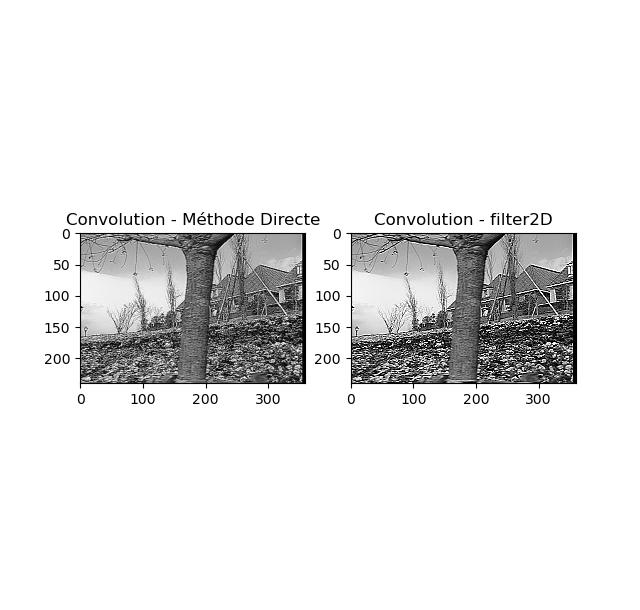
\includegraphics[trim= 0 130 0 130, clip = true, width=0.9\linewidth]{Images/Convolution.png}
		\caption{Résultats obtenus avec \textit{Convolution directe} e \textit{filter2D}}
		\label{fig:convolution}
	\end{figure}
	
	% ====================================================
	\begin{formal}
		\textbf{Q2 — Effet du noyau de convolution}
	\end{formal}
	
	Le noyau utilisé est :
	
	(Insérer la matrice)
	
	Ce noyau se caractérise par un coefficient central fort (+5) et par la soustraction des quatre voisins directs (-1). Cette configuration correspond à un filtre d’accentuation (sharpening filter).
	
	Dans une zone homogène, les pixels voisins ont des valeurs proches du pixel central. L’expression :
	
	$$
	5x_{centre} - \sum x_{voisins}
	$$
	
	reste donc approximativement égale à la valeur initiale, ce qui conserve l’intensité globale.
	
	En revanche, dans les zones où la variation spatiale est importante (contours, textures), la différence entre le pixel central et ses voisins est amplifiée. Le résultat est une augmentation du contraste local, ce qui rend les contours plus nets et plus visibles. Le noyau agit donc comme un opérateur de rehaussement de détails.
	
	% ====================================================
	\begin{formal}
		\textbf{Q3 — Calcul du gradient}
	\end{formal}
	
	Le calcul du gradient [figure \ref{fig:grad}] permet d’estimer les variations locales d’intensité et constitue la base de nombreux détecteurs de contours.
	
	Un opérateur simple peut être défini par :
	
	$$
	K_x = [-1\ 0\ 1]
	$$
	
	$$
	K_y = [-1\ 0\ 1]^T
	$$
	
	Après convolution avec ces noyaux, on obtient les composantes horizontale et verticale du gradient :
	
	$$
	I_x \quad \text{et} \quad I_y
	$$
	
	La norme du gradient est ensuite calculée pour chaque pixel :
	
	$$
	\|\nabla I\| = \sqrt{I_x^2 + I_y^2}
	$$
	
	\begin{figure}[H]
		\centering
		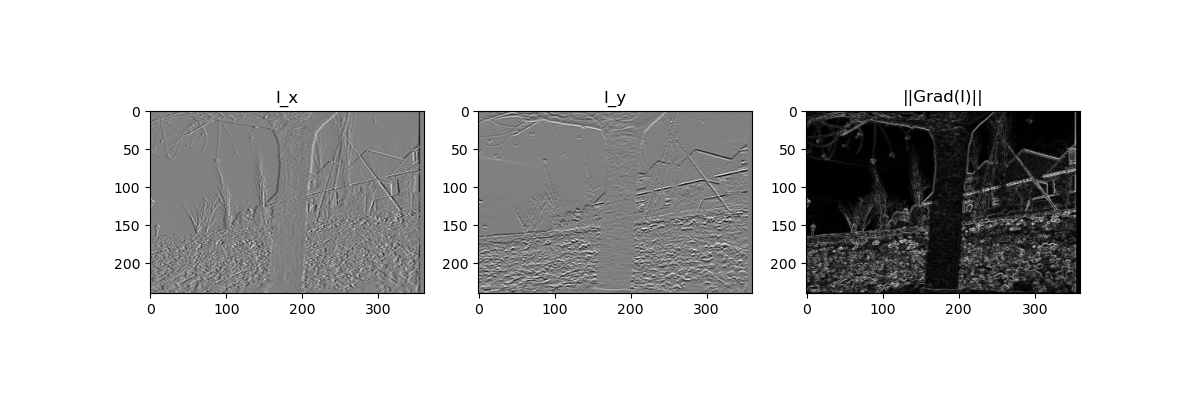
\includegraphics[trim= 70 20 80 20, clip = true, width=0.9\linewidth]{Images/Grad_Simple.png}
		\caption{Résultats obtenus avec le calcul du \textit{gradient}}
		\label{fig:grad}
	\end{figure}
	
	Cependant, ces noyaux simples sont sensibles au bruit. Pour améliorer la robustesse, on utilise le filtre de Sobel, qui intègre une pondération supplémentaire :
	
	$$
	K_x =
	\begin{bmatrix}
		-1 & 0 & 1 \\
		-2 & 0 & 2 \\
		-1 & 0 & 1
	\end{bmatrix}
	$$
	
	$$
	K_y =
	\begin{bmatrix}
		-1 & -2 & -1 \\
		0 & 0 & 0 \\
		1 & 2 & 1
	\end{bmatrix}
	$$
	
	Le filtre de Sobel [figure \ref{fig:Sobel}] combine dérivation et lissage, ce qui permet d’obtenir un gradient plus stable et moins sensible aux fluctuations locales. Les résultats expérimentaux montrent une meilleure définition des contours.
	
	Lors de l’affichage, il est indispensable de normaliser l’image résultante afin d’éviter des saturations ou des valeurs négatives incompatibles avec l’affichage en niveaux de gris.
	
	\begin{figure}[H]
		\centering
		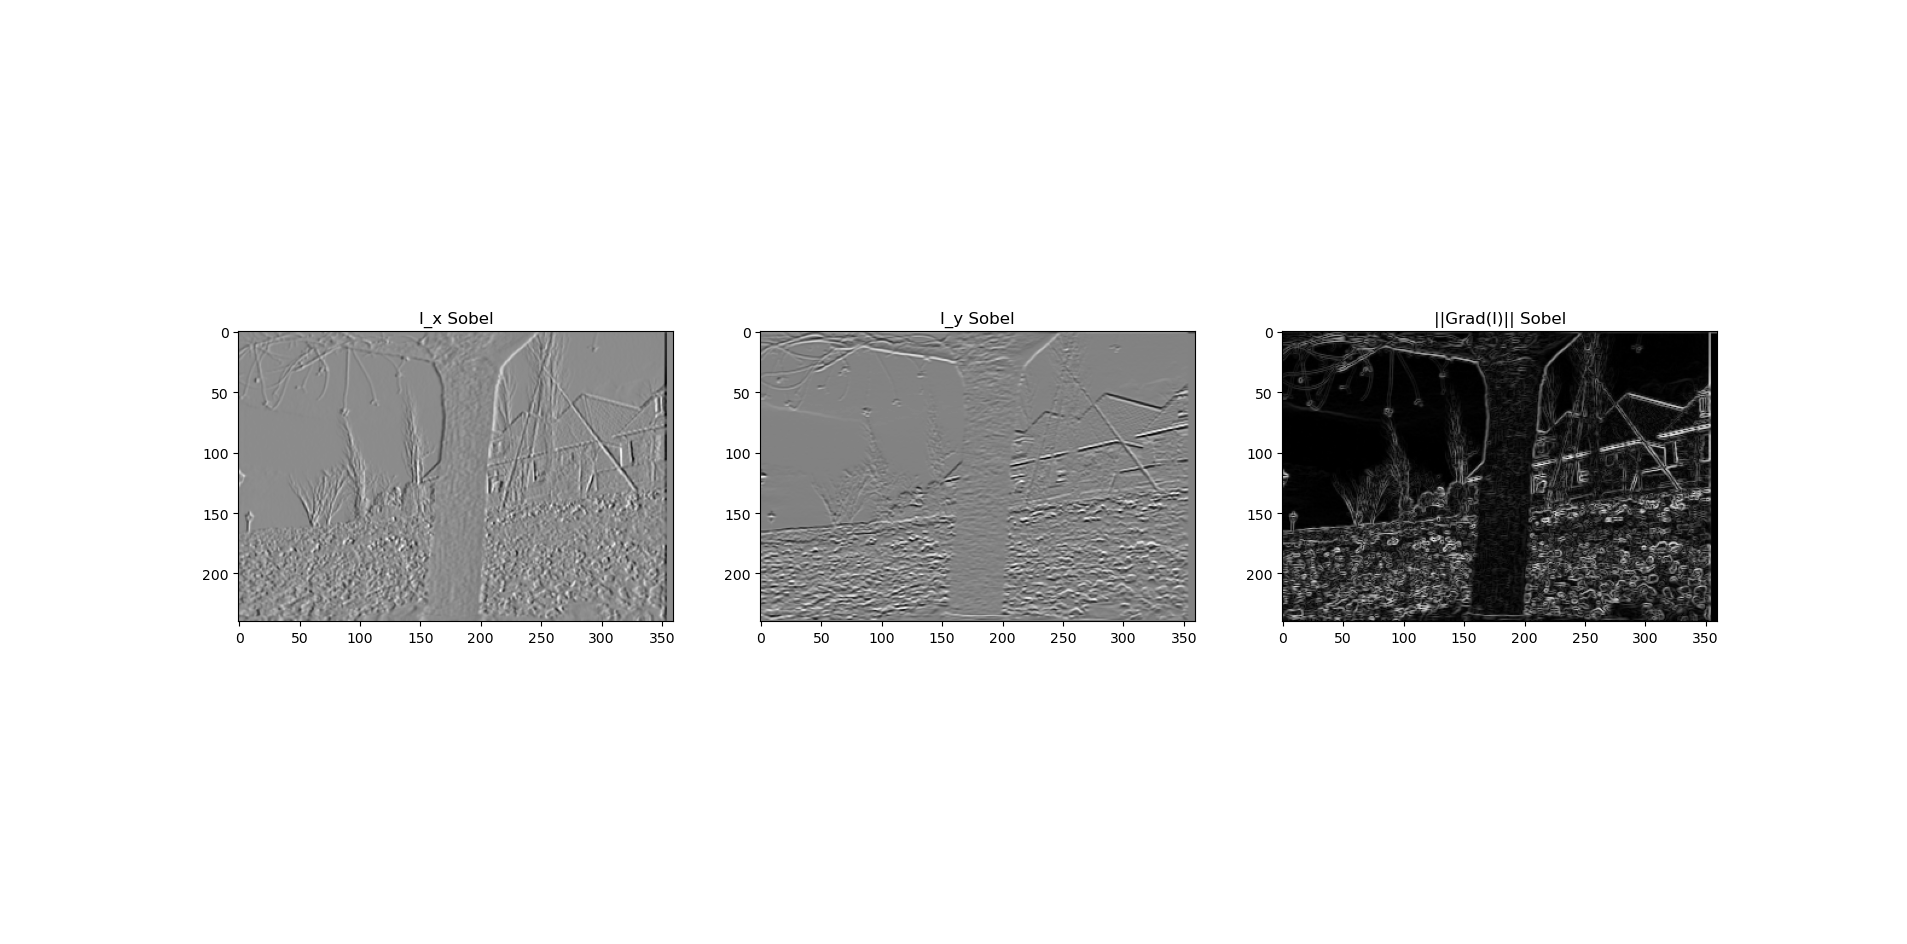
\includegraphics[trim= 100 140 100 150, clip = true, width=0.95\linewidth]{Images/Grad_Sobel.png}
		\caption{Résultats obtenus avec le \textit{filtre Sobel}}
		\label{fig:Sobel}
	\end{figure}
	
	
	% ====================================================
	% 3. DÉTECTEURS DE POINTS D’INTÉRÊT
	% ====================================================
	
	\section*{3. Détecteurs de points d’intérêt}
	
	\begin{formal}
		\textbf{Q4 — Détecteur de Harris}
	\end{formal}
	
	Le détecteur de Harris repose sur l’analyse locale des variations du gradient dans une fenêtre $W$. La matrice d’auto-corrélation est définie par :
	
	$$
	M =
	\begin{bmatrix}
		\sum_W I_x^2 & \sum_W I_x I_y \\
		\sum_W I_x I_y & \sum_W I_y^2
	\end{bmatrix}
	$$
	
	La fonction d’intérêt est donnée par :
	
	$$
	R = \det(M) - \alpha (\mathrm{tr}(M))^2
	$$
	
	Cette formulation permet de distinguer trois types de régions :
	
	\begin{itemize}
		\item[-] Régions plates : gradients faibles $\Rightarrow$ $R$ faible
		\item[-] Arêtes : un gradient dominant $\Rightarrow$ $R$ modéré 
		\item[-] Coins : gradients forts dans deux directions $\Rightarrow$ $R$ élevé  
	\end{itemize}
	
	Les maxima locaux de $R$ correspondent aux points d’intérêt.
	
	Afin d’éviter la sélection de plusieurs pixels adjacents appartenant au même coin, une dilatation morphologique est appliquée. Cette opération permet de conserver uniquement les maxima locaux dans un voisinage donné.
	% ====================================================
	\begin{formal}
		\textbf{Q5 — Analyse des paramètres du détecteur de Harris}
	\end{formal}
	
	Le détecteur de Harris dépend de plusieurs paramètres influençant directement la qualité et la stabilité des points détectés.
	
	Le premier paramètre essentiel est la taille de la fenêtre [figure \ref{fig:harris_fenetre}] $W$ utilisée pour calculer la matrice $M$. Cette fenêtre définit l’échelle locale d’analyse. Une petite fenêtre permet une localisation spatiale très précise mais rend le détecteur plus sensible au bruit, car les gradients locaux peuvent être fortement influencés par des fluctuations d’intensité. À l’inverse, une fenêtre plus grande introduit un effet de lissage spatial : les gradients sont intégrés sur une région plus étendue, ce qui améliore la robustesse au bruit mais réduit la précision de localisation.
	
	\begin{figure}[H]
		\centering
		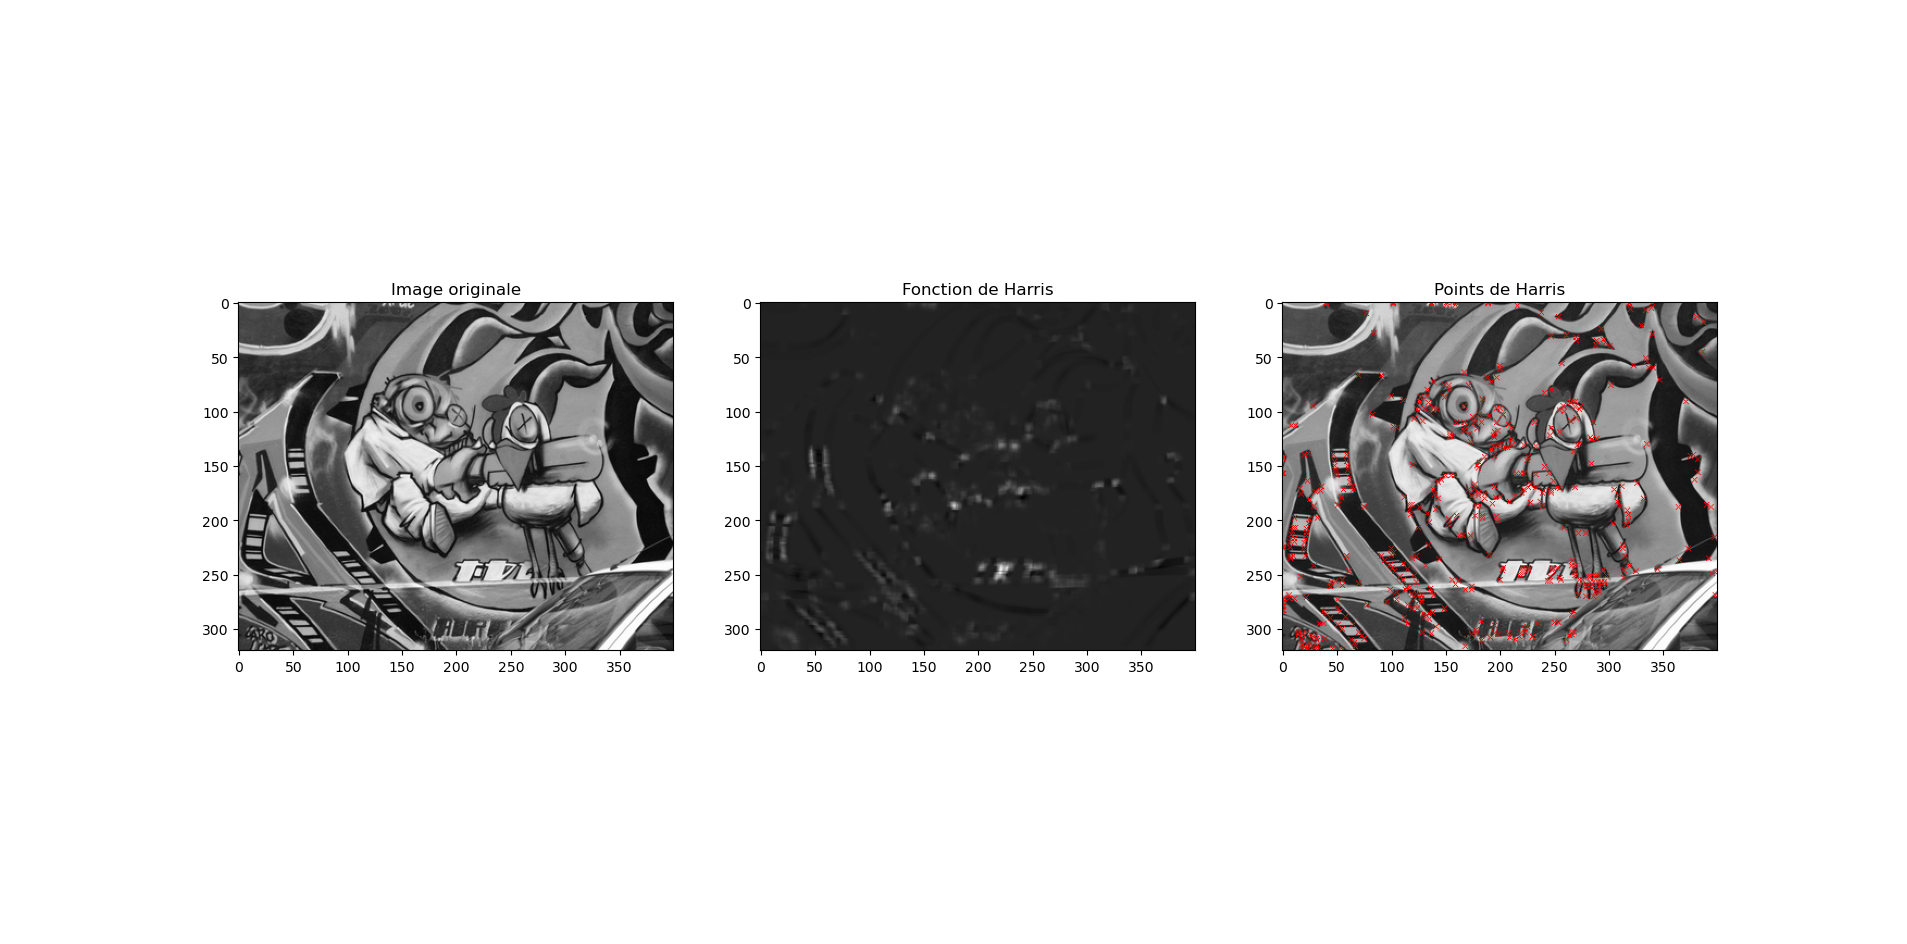
\includegraphics[trim= 125 130 120 130, clip = true, width=0.9\linewidth]{Images/Harris_fenetre8.png}
		\caption{Résultats obtenus avec une fenêtre de taille 8 }
		\label{fig:harris_fenetre}
	\end{figure}
	
	Le paramètre $\alpha$ joue un rôle fondamental dans la fonction de décision :
	
	$$
	R = \det(M) - \alpha (\mathrm{tr}(M))^2
	$$
	
	\begin{figure}[H]
		\centering
		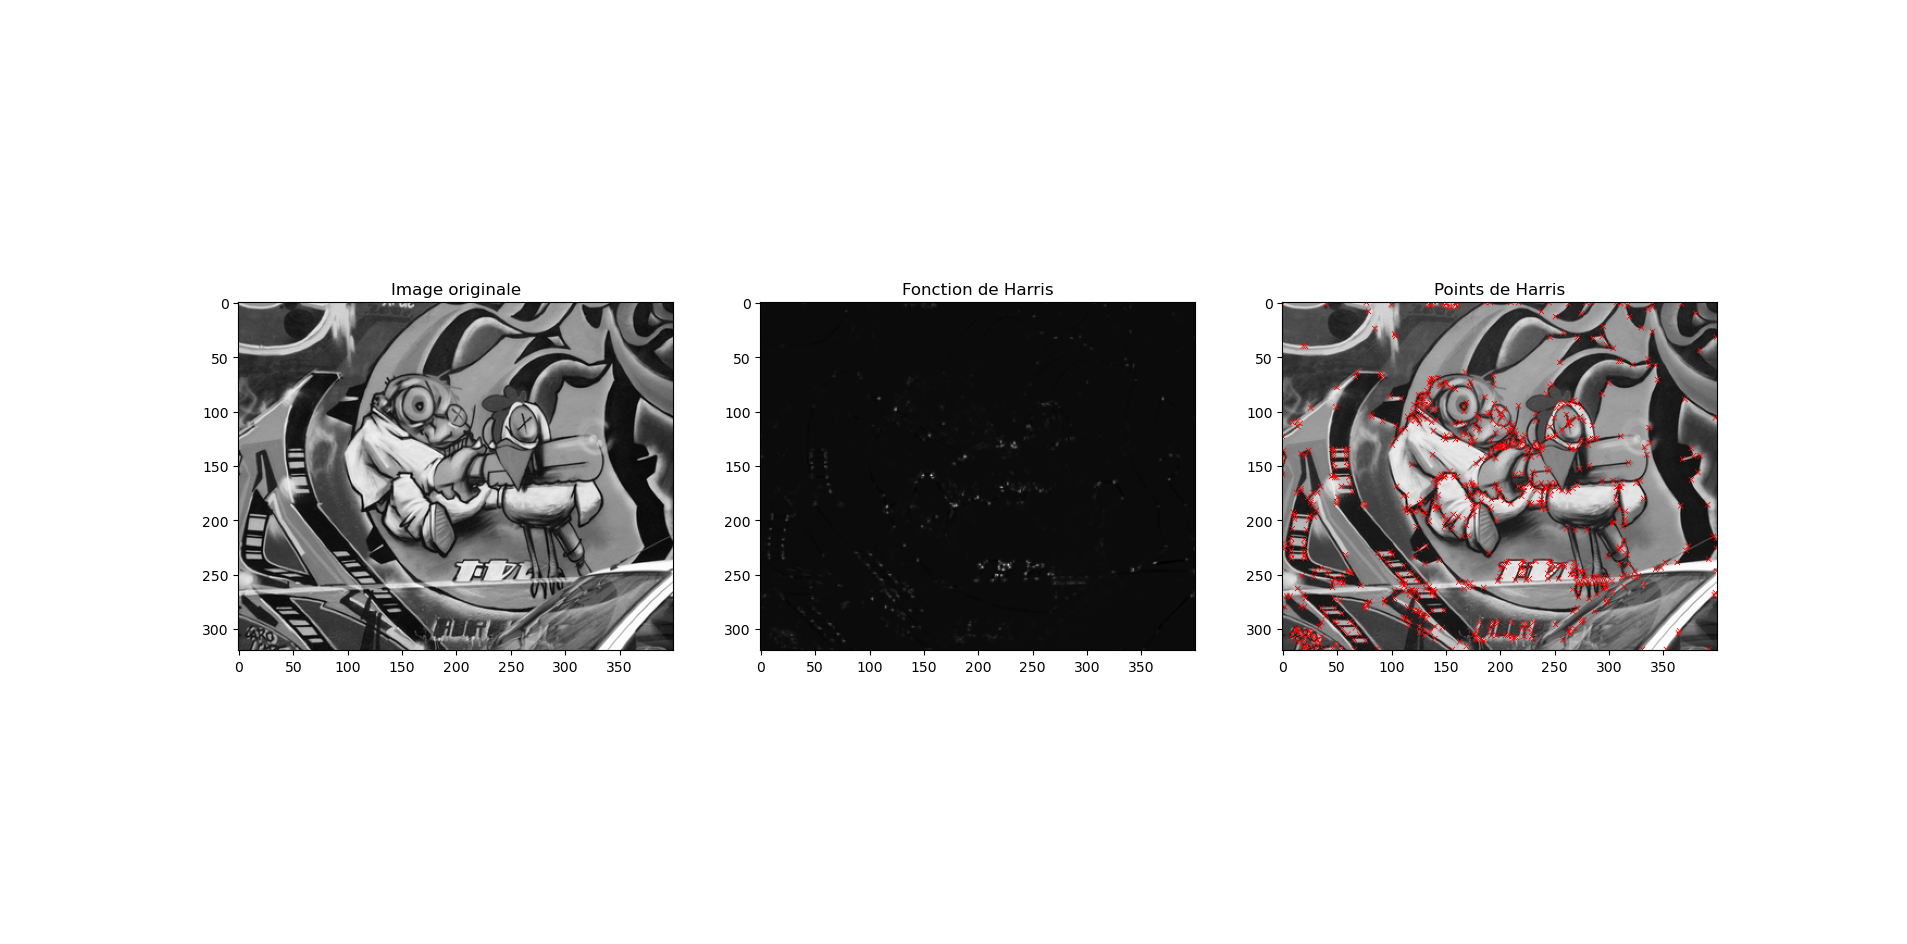
\includegraphics[trim= 125 180 120 200, clip = true, width=0.9\linewidth]{Images/Harris_alpha001.png}
		\caption{Résultats obtenus avec $\alpha = 0.001$ }
		\label{fig:harris_alpha001}
	\end{figure}
	
	Ce terme pondère l’importance relative de la trace par rapport au déterminant. Un $\alpha$ faible [figure \ref{fig:harris_alpha001}] réduit la pénalisation des arêtes, ce qui conduit à la détection d’un plus grand nombre de points, y compris des structures ambiguës. Un $\alpha$ plus élevé [figure \ref{fig:harris_alpha01}] renforce la sélectivité du détecteur en favorisant les régions où les variations sont significatives dans deux directions orthogonales. En pratique, $\alpha$ est généralement compris entre 0.04 et 0.06 [figure \ref{fig:harris_alpha005}].
	
	\begin{figure}[H]
		\centering
		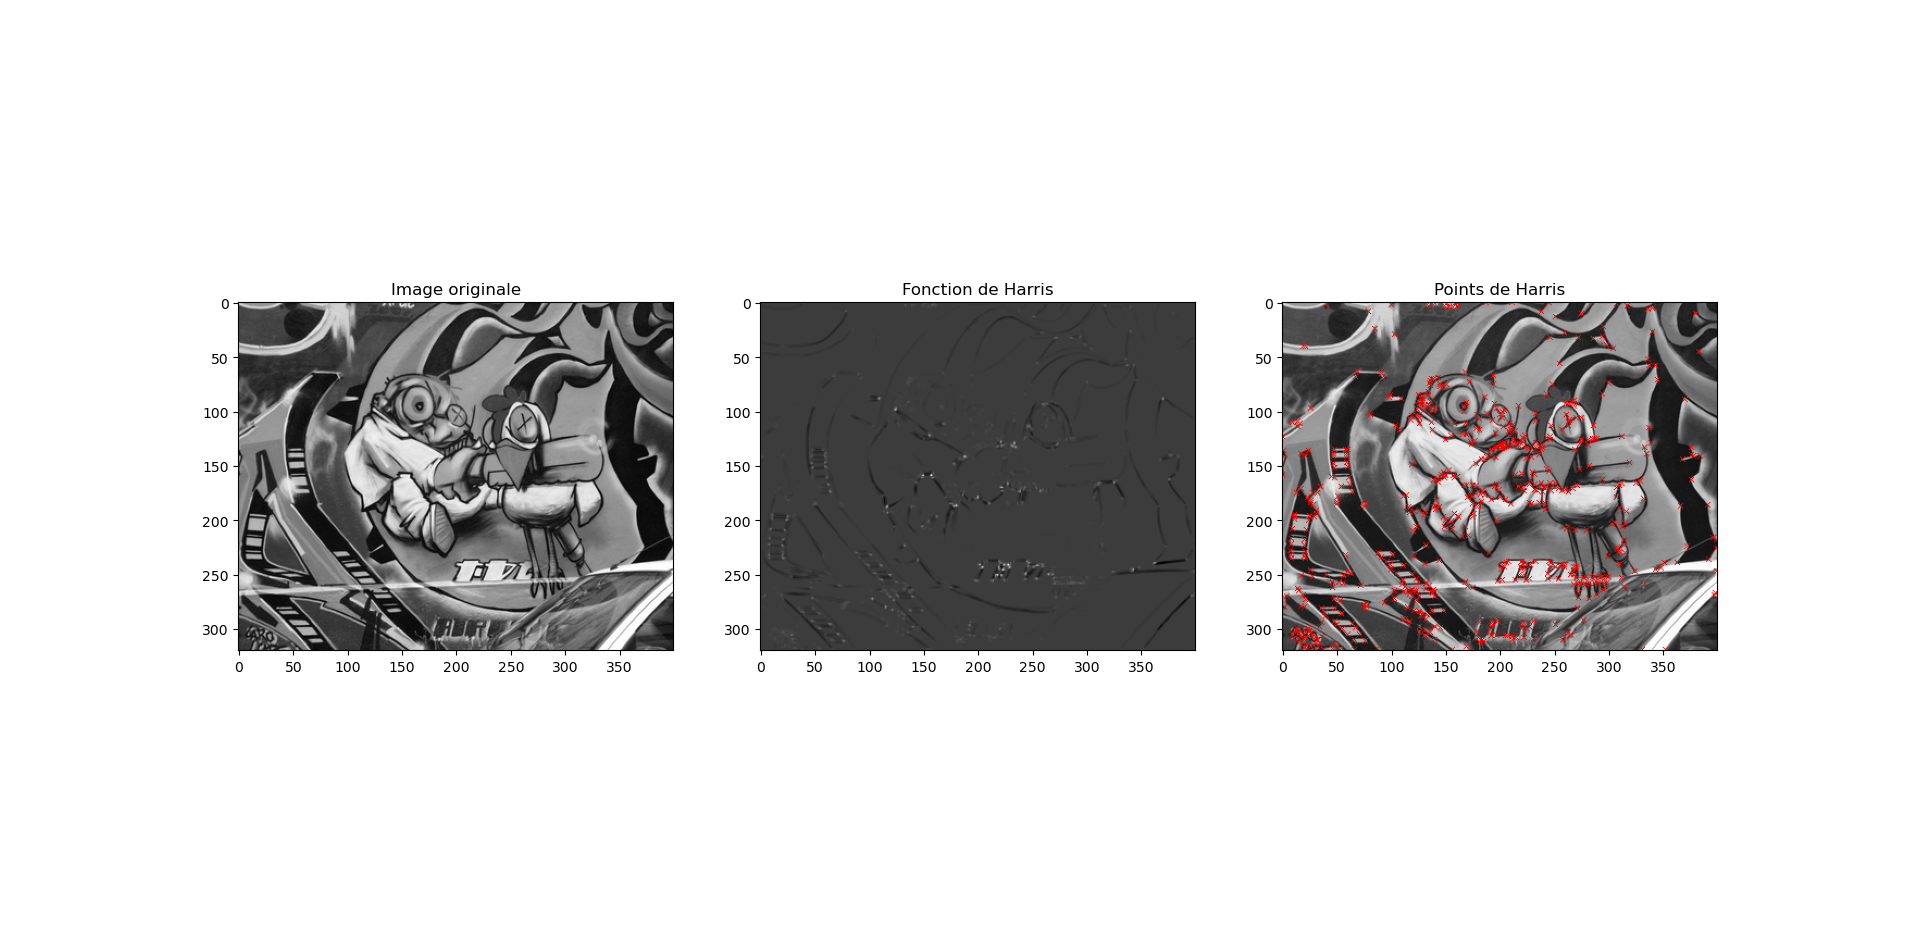
\includegraphics[trim= 125 180 120 200, clip = true, width=0.9\linewidth]{Images/Harris_alpha005.png}
		\caption{Résultats obtenus avec $\alpha = 0.005$ }
		\label{fig:harris_alpha005}
	\end{figure}
	
	Afin d’assurer une invariance partielle au changement d’échelle, une stratégie multi-échelle peut être adoptée. Elle consiste à construire une pyramide gaussienne de l’image et à appliquer le détecteur de Harris à chaque niveau. Les points détectés à différentes résolutions correspondent alors à des structures observées à différentes échelles spatiales.
	
	\begin{figure}[H]
		\centering
		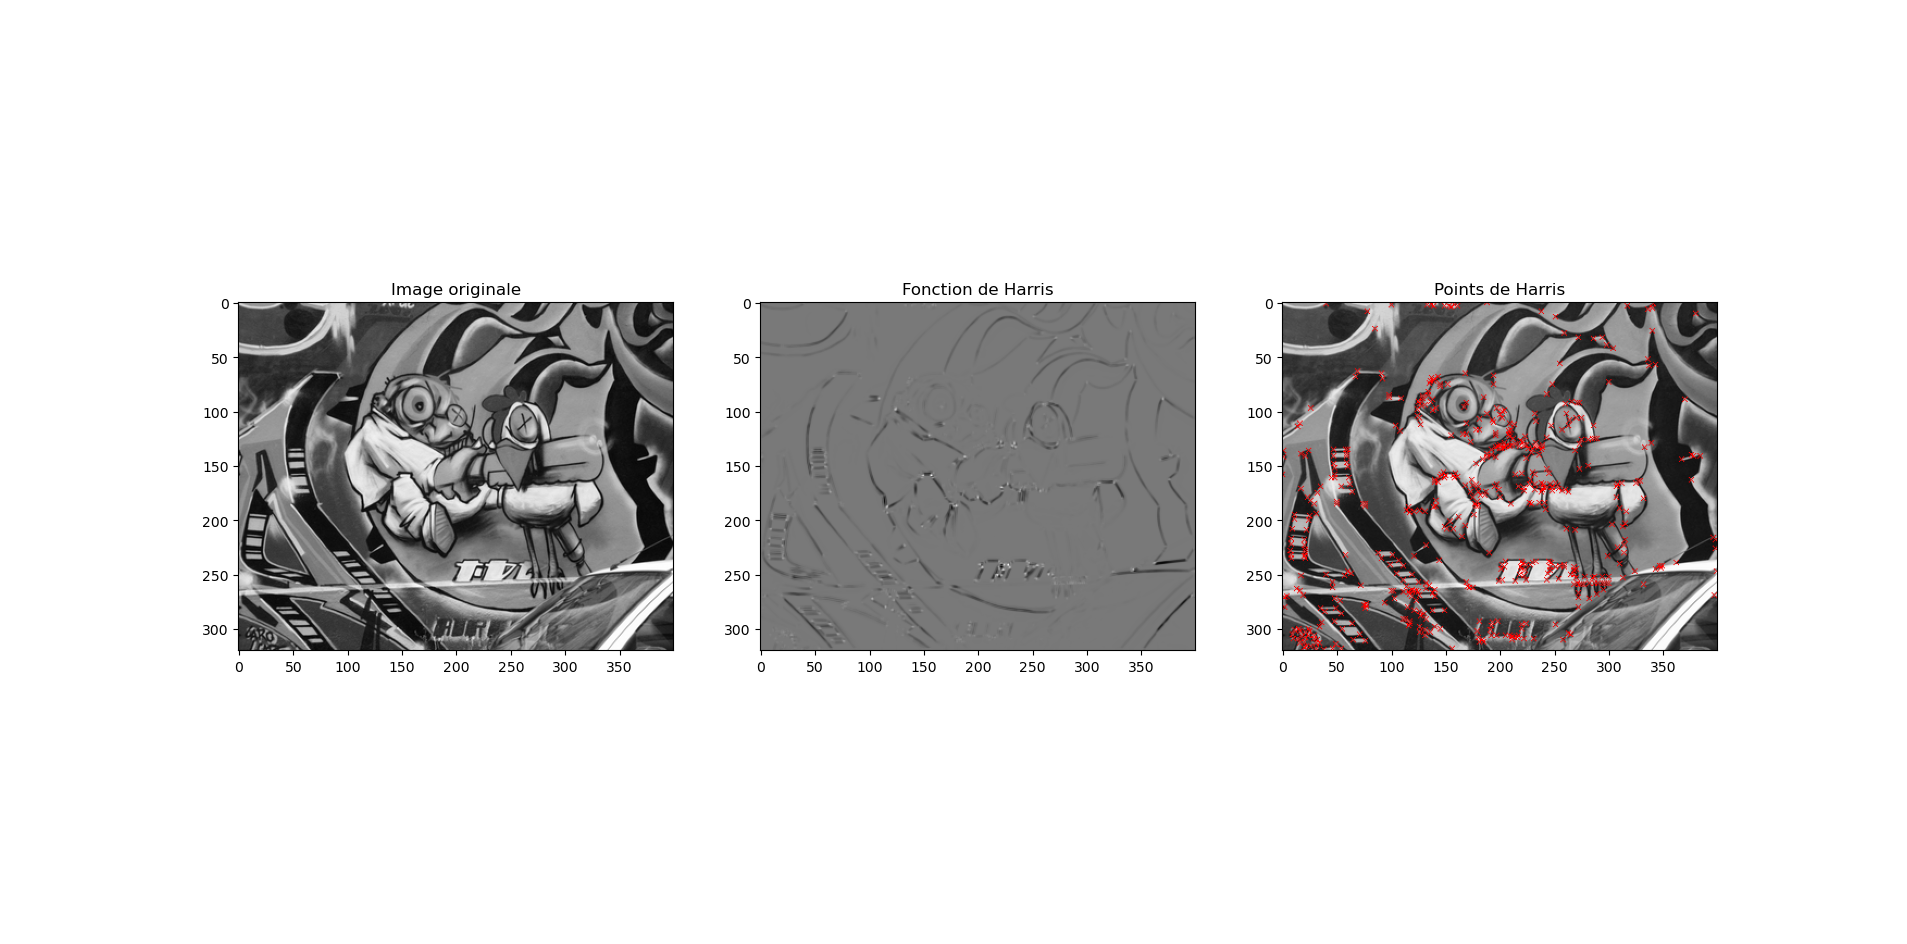
\includegraphics[trim= 125 180 120 200, clip = true, width=0.9\linewidth]{Images/Harris_alpha01.png}
		\caption{Résultats obtenus avec $\alpha = 0.1$ }
		\label{fig:harris_alpha01}
	\end{figure}
	
	% ====================================================
	\begin{formal}
		\textbf{Q6 — Analyse approfondie de ORB et KAZE}
	\end{formal}
	
	\textbf{ORB (Oriented FAST and Rotated BRIEF)}
	
	ORB [figure \ref{fig:orb}] est une méthode conçue pour fournir une alternative rapide et libre de droits à SIFT et SURF. Elle combine un détecteur de points d’intérêt (FAST) et un descripteur binaire (BRIEF), enrichis par des mécanismes assurant une invariance en rotation et une robustesse multi-échelle.
	
	\begin{figure}
		\centering
		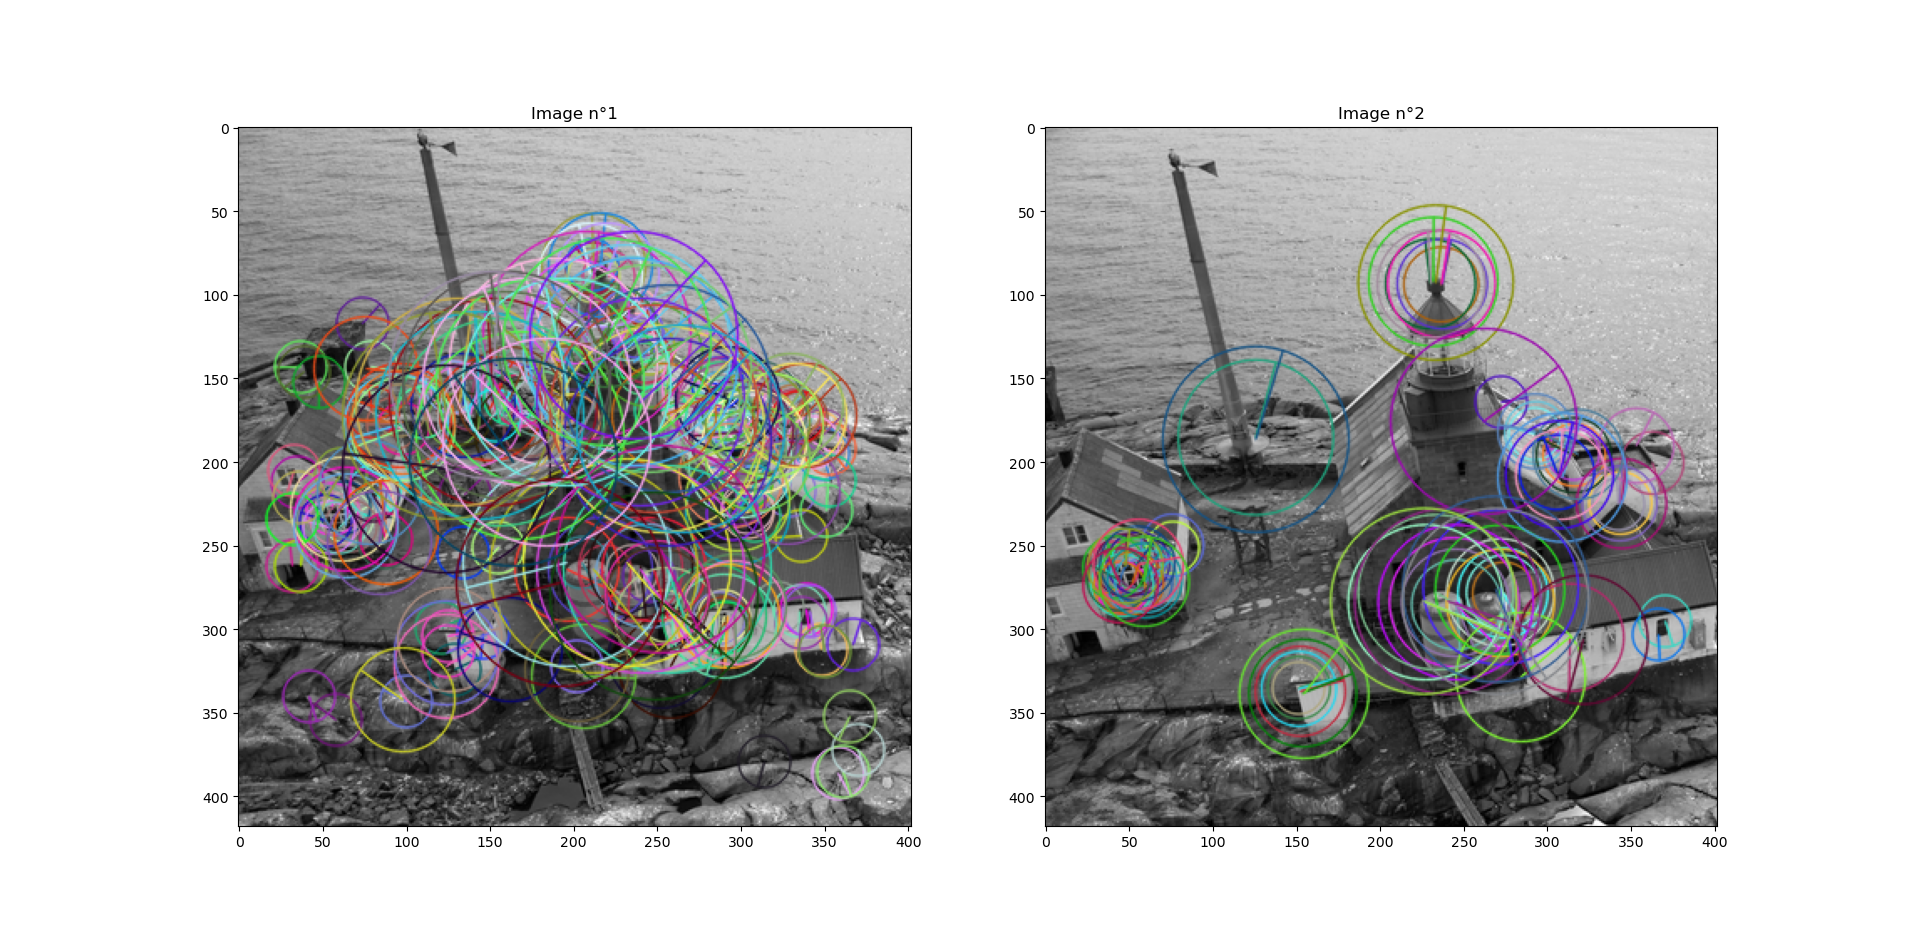
\includegraphics[trim= 30 20 30 20, clip = true, width=0.8\linewidth]{Images/ORB.png}
		\caption{Résultats obtenus avec le méthode ORB}
		\label{fig:orb}
	\end{figure}
	
	Le détecteur FAST (Features from Accelerated Segment Test) identifie les coins en examinant un cercle de 16 pixels autour d’un pixel candidat. Un pixel est considéré comme coin si un ensemble contigu de pixels du cercle est significativement plus clair ou plus sombre que le pixel central selon un seuil donné. Cette stratégie repose sur un test binaire rapide, optimisé par une structure en arbre décisionnel.
	
	Cependant, FAST n’est pas intrinsèquement invariant à l’échelle. ORB introduit donc une pyramide d’images multi-échelle (Gaussian pyramid). À chaque niveau de la pyramide, FAST est appliqué indépendamment. Cela permet de détecter des points correspondant à différentes tailles d’objets dans l’image originale. Cette pyramide constitue une représentation discrète de l’espace d’échelle.
	
	ORB ajoute également une estimation d’orientation pour chaque point détecté. L’orientation est calculée à partir des moments d’intensité dans un voisinage local, permettant de définir un angle dominant. Cette orientation est ensuite utilisée pour « tourner » le descripteur BRIEF afin d’assurer l’invariance en rotation.
	
	Le descripteur BRIEF (Binary Robust Independent Elementary Features) repose sur des comparaisons binaires entre paires de pixels dans un patch local. Chaque comparaison génère un bit selon :
	
	$$
	\tau(p; x, y) =
	\begin{cases}
		1 & \text{si } I(x) < I(y) \\
		0 & \text{sinon}
	\end{cases}
	$$
	
	Un ensemble de telles comparaisons forme un vecteur binaire. La distance entre descripteurs est calculée via la distance de Hamming, ce qui permet un appariement extrêmement rapide.
	
	ORB optimise la sélection des paires de points afin de maximiser la variance et de minimiser la corrélation entre tests binaires, améliorant ainsi le pouvoir discriminant.
	
	\begin{figure}[H]
		\centering
		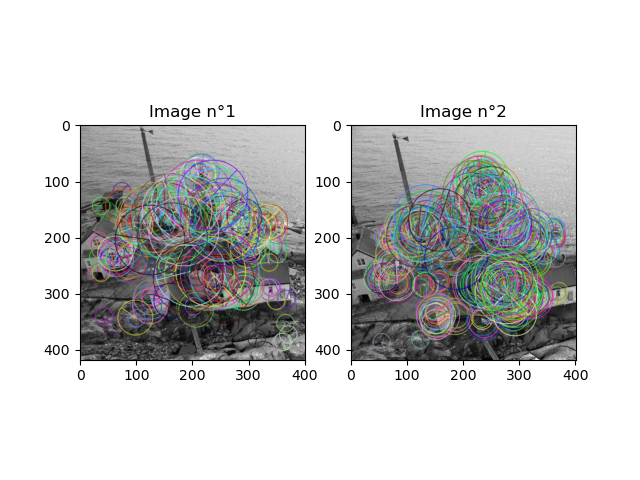
\includegraphics[trim= 0 50 0 50, clip = true, width=0.75\linewidth]{Images/ORBN_500.png}
		\caption{Méthode ORB avec deux fois le nombre de points}
		\label{fig:orb500}
	\end{figure}
	
	\textbf{KAZE}
	
	Contrairement à ORB, KAZE [figure \ref{fig:kaze}] repose sur une construction non linéaire de l’espace d’échelle.
	
	Les méthodes classiques comme SIFT utilisent un espace d’échelle gaussien défini par la solution de l’équation de la chaleur :
	
	$$
	\frac{\partial L}{\partial t} = \Delta L
	$$
	
	où $\Delta$ est le Laplacien. Cette diffusion est linéaire et isotrope : elle lisse uniformément l’image dans toutes les directions, ce qui peut atténuer les contours importants.
	
	\begin{figure}[H]
		\centering
		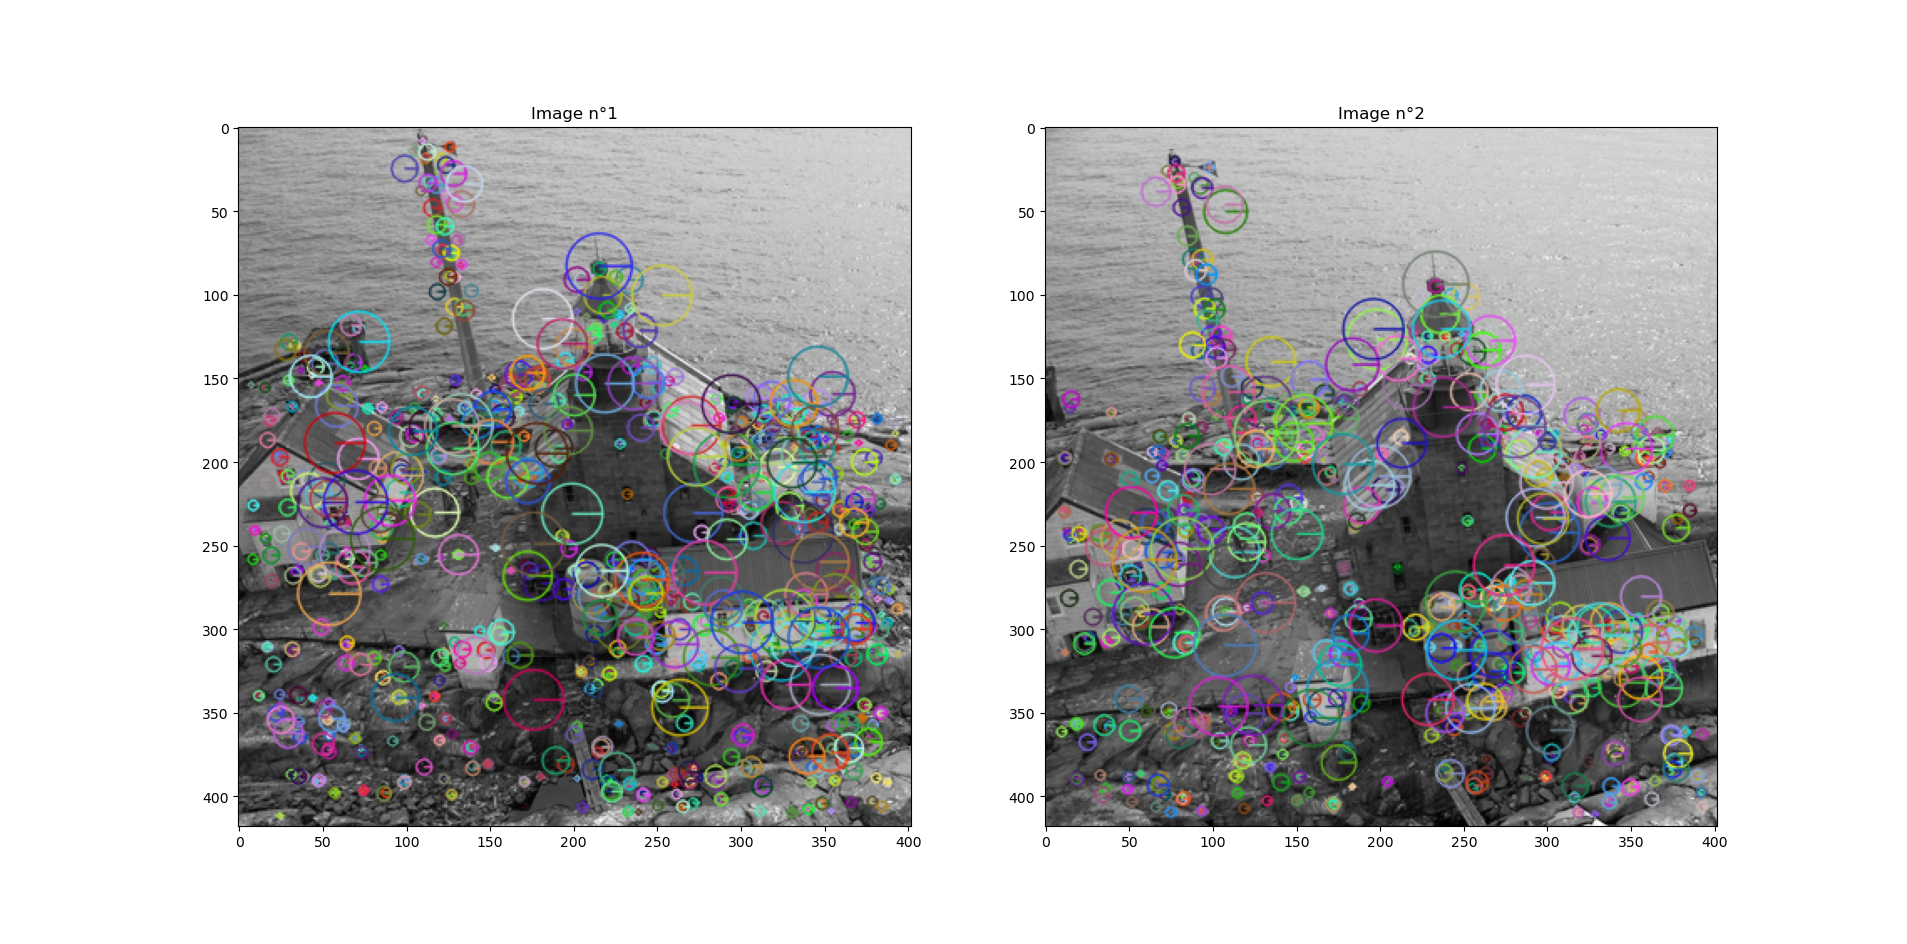
\includegraphics[trim= 30 20 30 20, clip = true, width=0.9\linewidth]{Images/Kaze.png}
		\caption{Résultats obtenus avec le méthode KAZE}
		\label{fig:kaze}
	\end{figure}
	
	KAZE introduit un espace d’échelle non gaussien basé sur une diffusion non linéaire inspirée du modèle de Perona-Malik :
	
	$$
	\frac{\partial L}{\partial t} = \nabla \cdot (c(x,y,t)\nabla L)
	$$
	
	où le coefficient de diffusion $c(x,y,t)$ dépend du gradient local. Lorsque le gradient est faible (zone homogène), la diffusion est forte et le lissage important. Lorsque le gradient est élevé (près d’un contour), la diffusion est réduite afin de préserver les structures significatives.
	
	Ce mécanisme permet de construire un espace d’échelle adaptatif qui respecte mieux les discontinuités importantes de l’image.
	
	L’implémentation numérique repose sur des schémas de diffusion accélérés (AOS — Additive Operator Splitting), garantissant stabilité et efficacité.
	
	Les points d’intérêt sont ensuite détectés via l’analyse du déterminant de la matrice Hessienne dans cet espace d’échelle non linéaire. Le descripteur associé est généralement un vecteur flottant basé sur des histogrammes locaux de gradients, ce qui le rend plus discriminant mais plus coûteux en calcul que les descripteurs binaires.
	
	Ainsi, ORB privilégie la rapidité et l’efficacité computationnelle, tandis que KAZE favorise la robustesse structurelle et la préservation des contours à travers une modélisation physique plus avancée de la diffusion.
	
	% ====================================================
	\begin{formal}
		\textbf{Q8 — Méthodes d’appariement}
	\end{formal}
	
	L’appariement des descripteurs repose sur la recherche des plus proches voisins dans l’espace des caractéristiques.
	
	La méthode CrossCheck [figures \ref{fig:kaze_CrossCheck} et \ref{fig:orb_CrossCheck}] impose une contrainte de correspondance mutuelle : un point $p_1$ de l’image 1 correspond à $p_2$ dans l’image 2 si et seulement si $p_2$ considère également $p_1$ comme son plus proche voisin. Cette stratégie est simple mais restrictive.
	
	\begin{figure}[H]
		\centering
		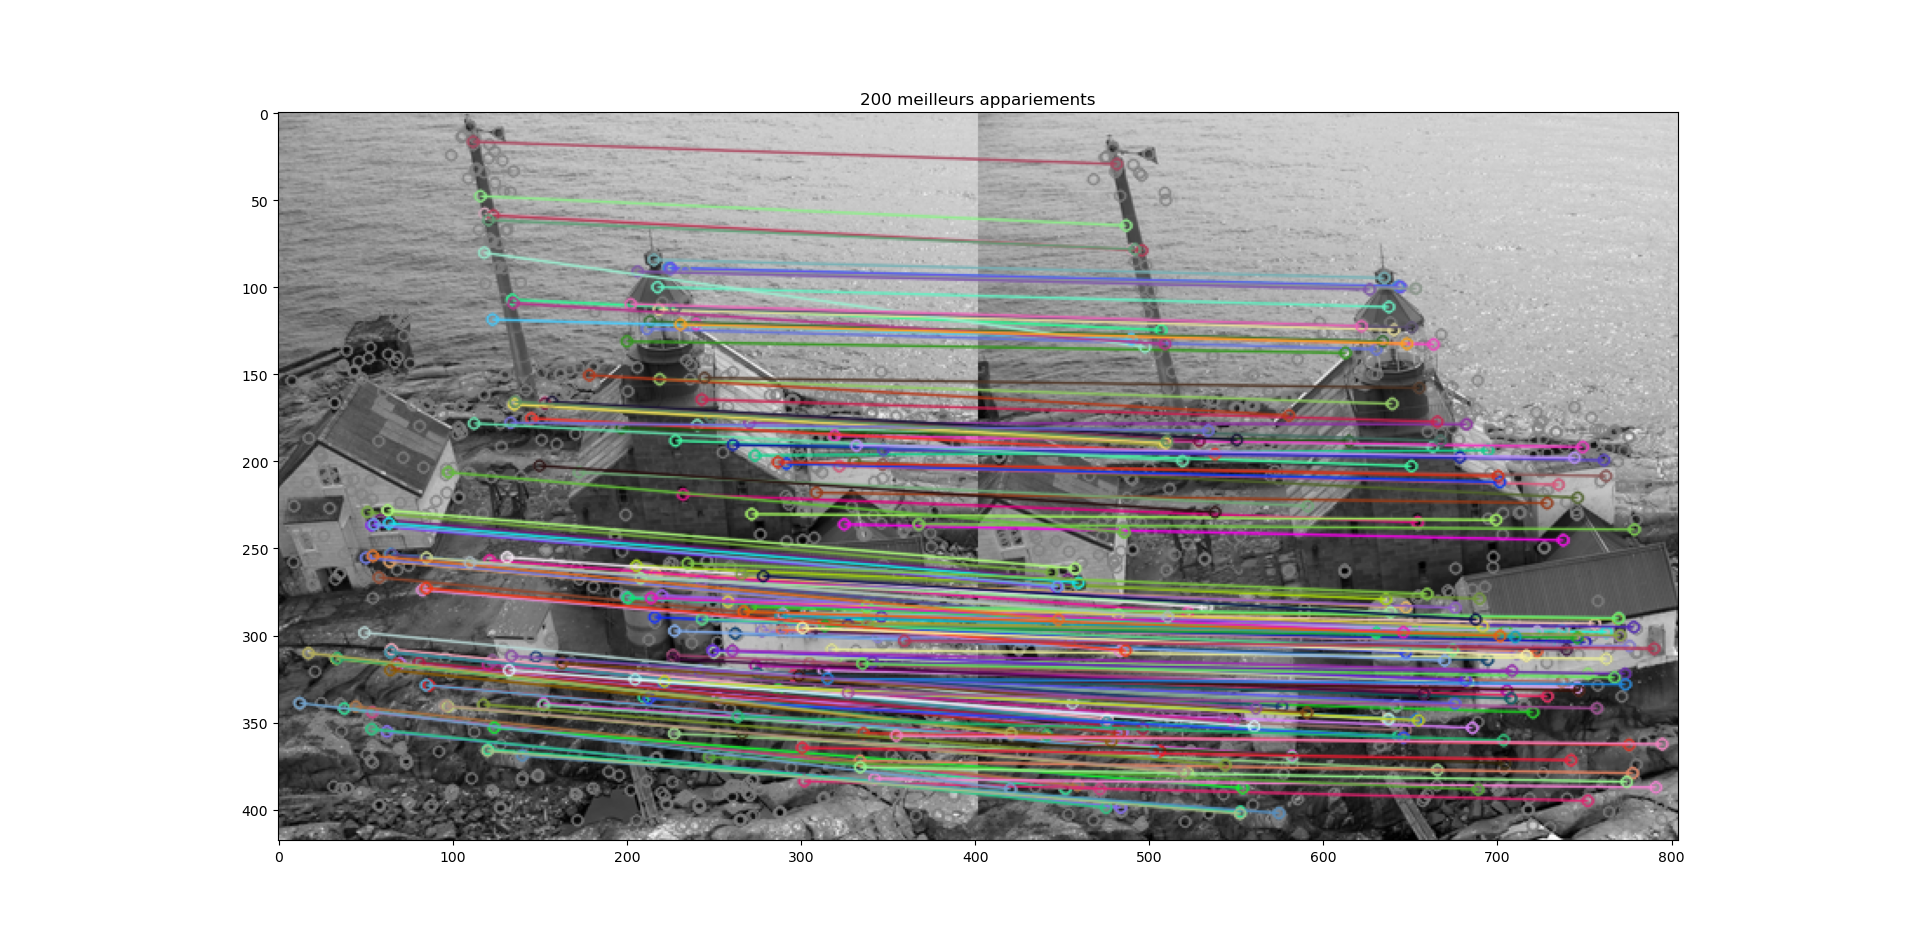
\includegraphics[trim= 50 40 50 40, clip = true, width=0.9\linewidth]{Images/Kaze_CrossCheck.png}
		\caption{Résultats obtenus avec le méthode \textit{KAZE} et \textit{CrossCheck}}
		\label{fig:kaze_CrossCheck}
	\end{figure}
	\begin{figure}[H]
		\centering
		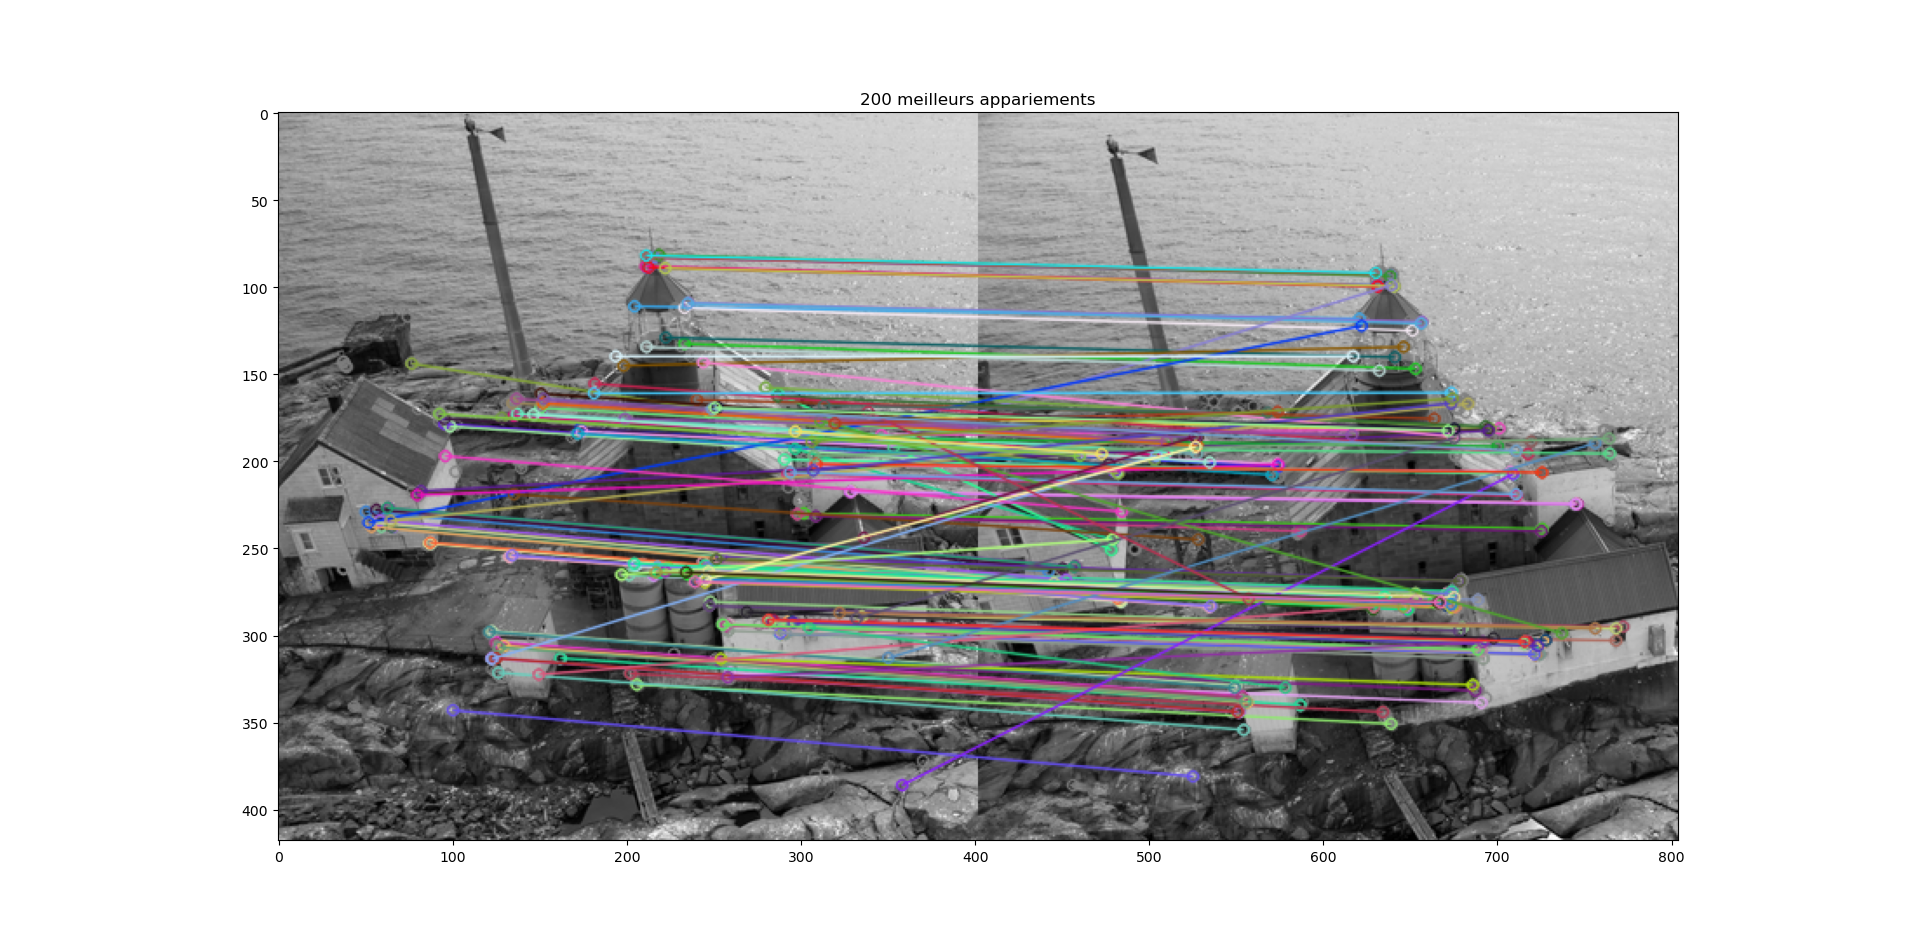
\includegraphics[trim= 50 40 50 40, clip = true, width=0.9\linewidth]{Images/ORB_CrossCheck.png}
		\caption{Résultats obtenus avec le méthode \textit{ORB} et \textit{CrossCheck}}
		\label{fig:orb_CrossCheck}
	\end{figure}
	
	Le Ratio Test proposé par Lowe consiste à comparer la distance au premier voisin $d_1$ avec celle au second voisin $d_2$. Si :
	
	$$
	\frac{d_1}{d_2} < \tau
	$$
	
	alors la correspondance est considérée comme fiable. Cette approche permet d’éliminer les correspondances ambiguës dans les régions répétitives.
	
	\begin{figure}[H]
		\centering
		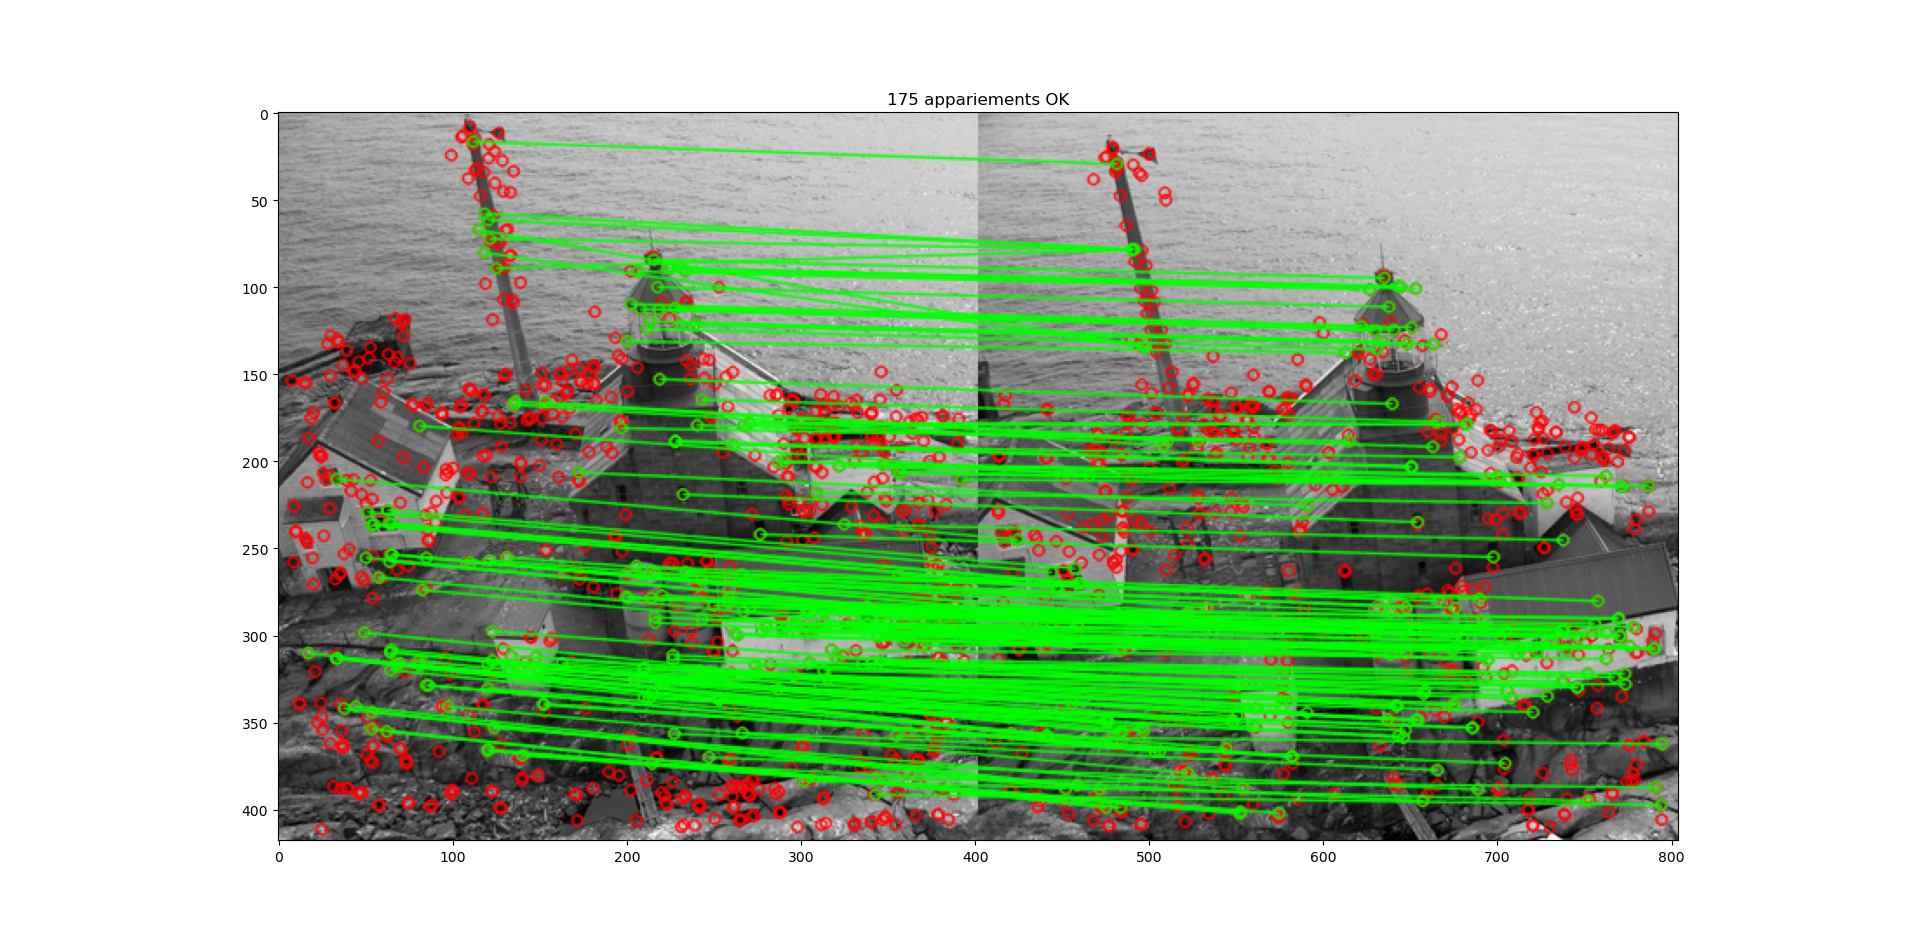
\includegraphics[trim= 50 40 50 40, clip = true, width=0.9\linewidth]{Images/Kaze_Ratio.png}
		\caption{Résultats obtenus avec le méthode \textit{KAZE} et \textit{Ratio}}
		\label{fig:kaze_Ratio}
	\end{figure}
	\begin{figure}[H]
		\centering
		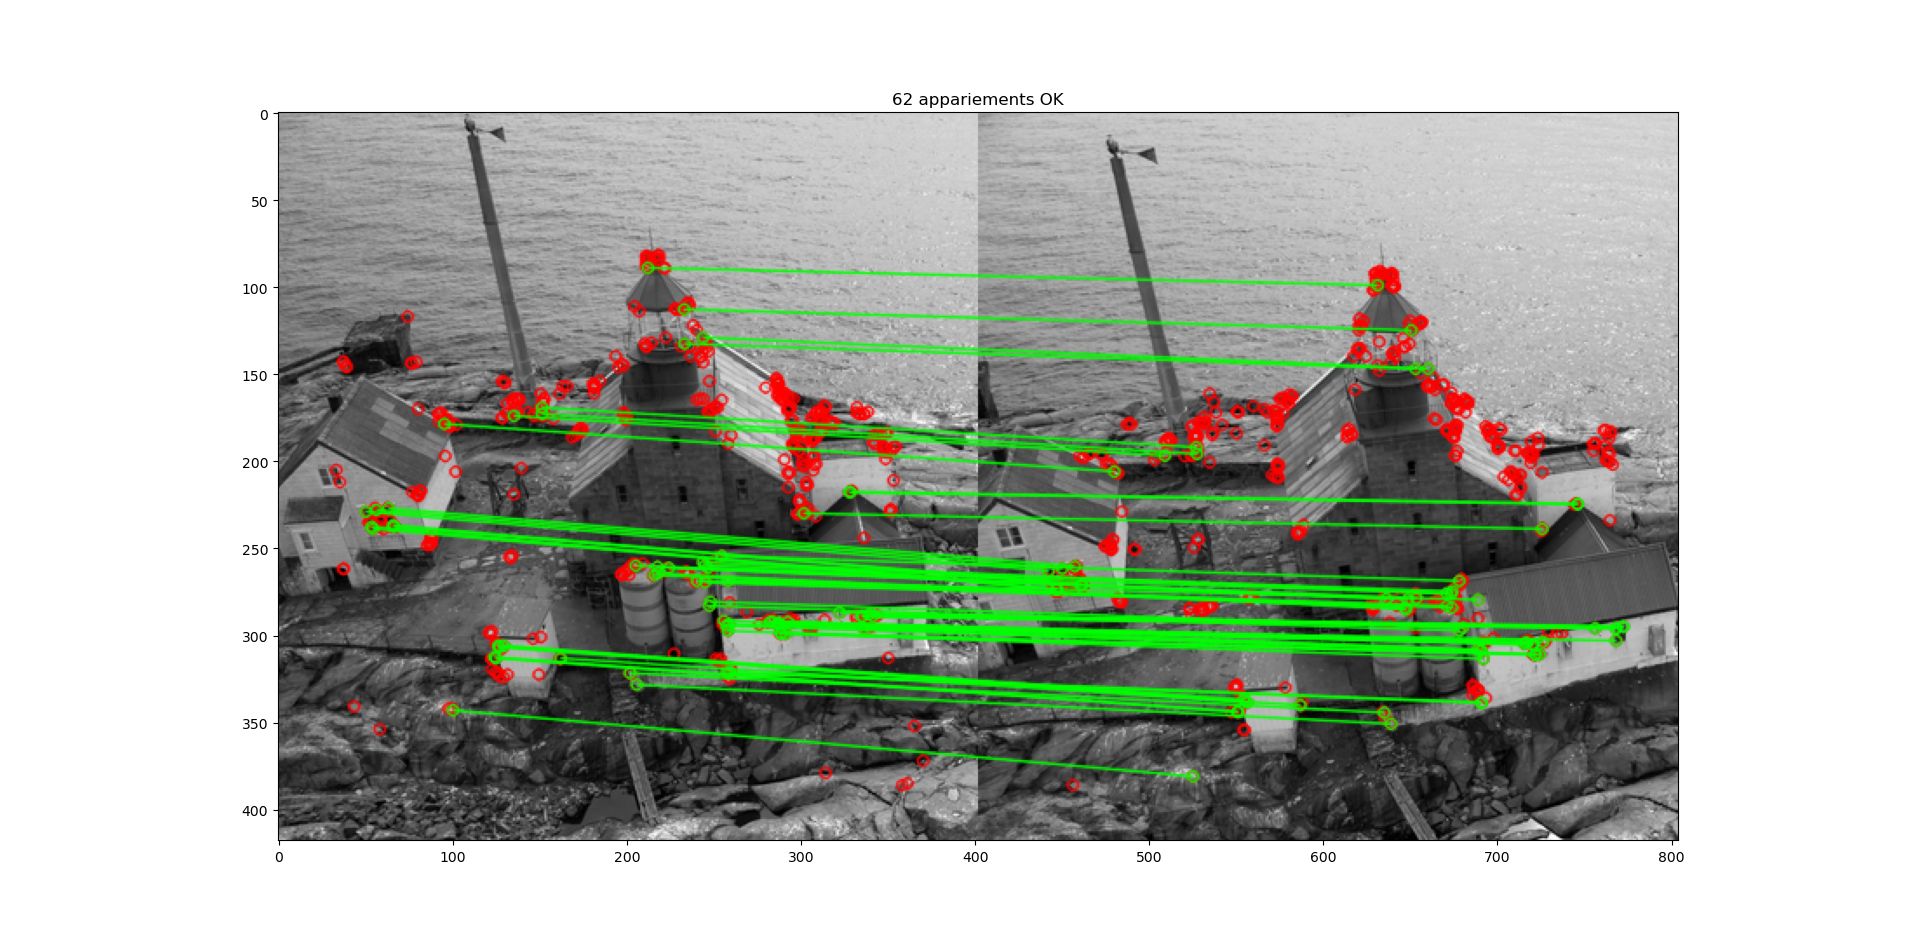
\includegraphics[trim= 50 40 50 40, clip = true, width=0.9\linewidth]{Images/ORB_Ratio.png}
		\caption{Résultats obtenus avec le méthode \textit{ORB} et \textit{Ratio}}
		\label{fig:orb_Ratio}
	\end{figure}
	
	FLANN (Fast Library for Approximate Nearest Neighbors) utilise des structures d’indexation comme les arbres KD ou les arbres hiérarchiques afin d’accélérer la recherche dans des espaces de grande dimension.
	
	\begin{figure}[H]
		\centering
		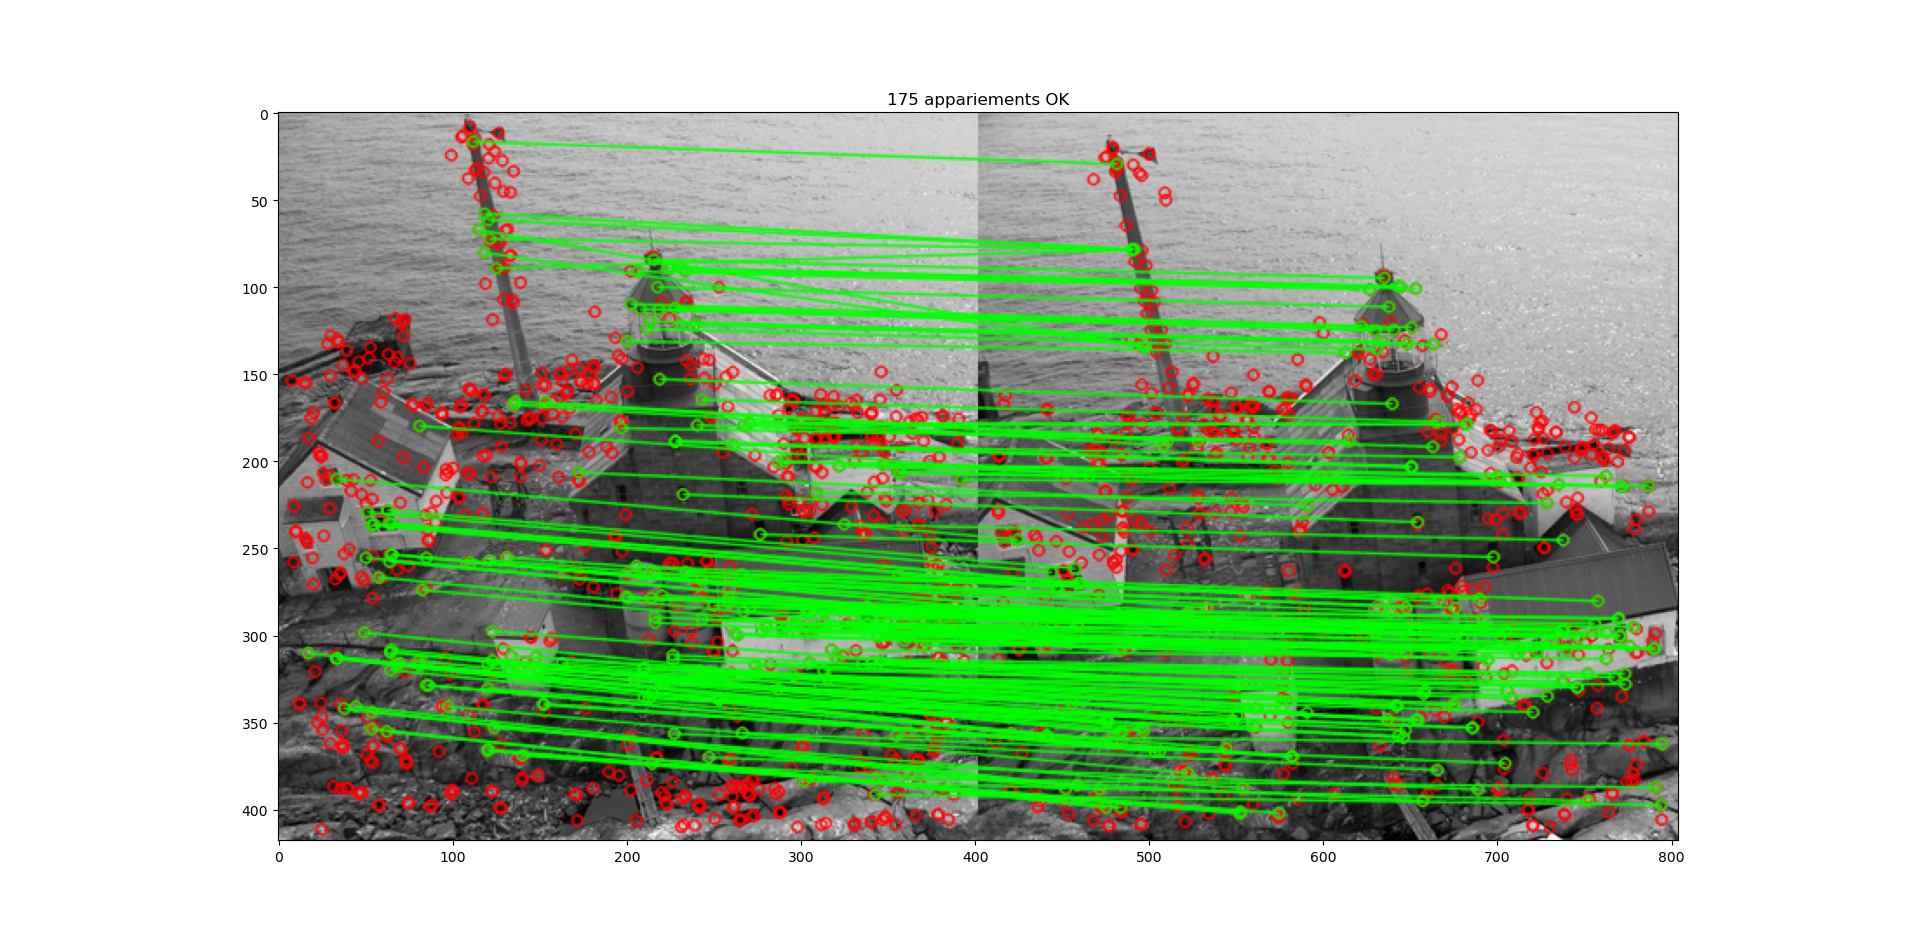
\includegraphics[trim= 50 40 50 40, clip = true, width=0.9\linewidth]{Images/Kaze_FLANN.png}
		\caption{Résultats obtenus avec le méthode \textit{KAZE} et \textit{FLANN}}
		\label{fig:kaze_Flann}
	\end{figure}
	\begin{figure}[H]
		\centering
		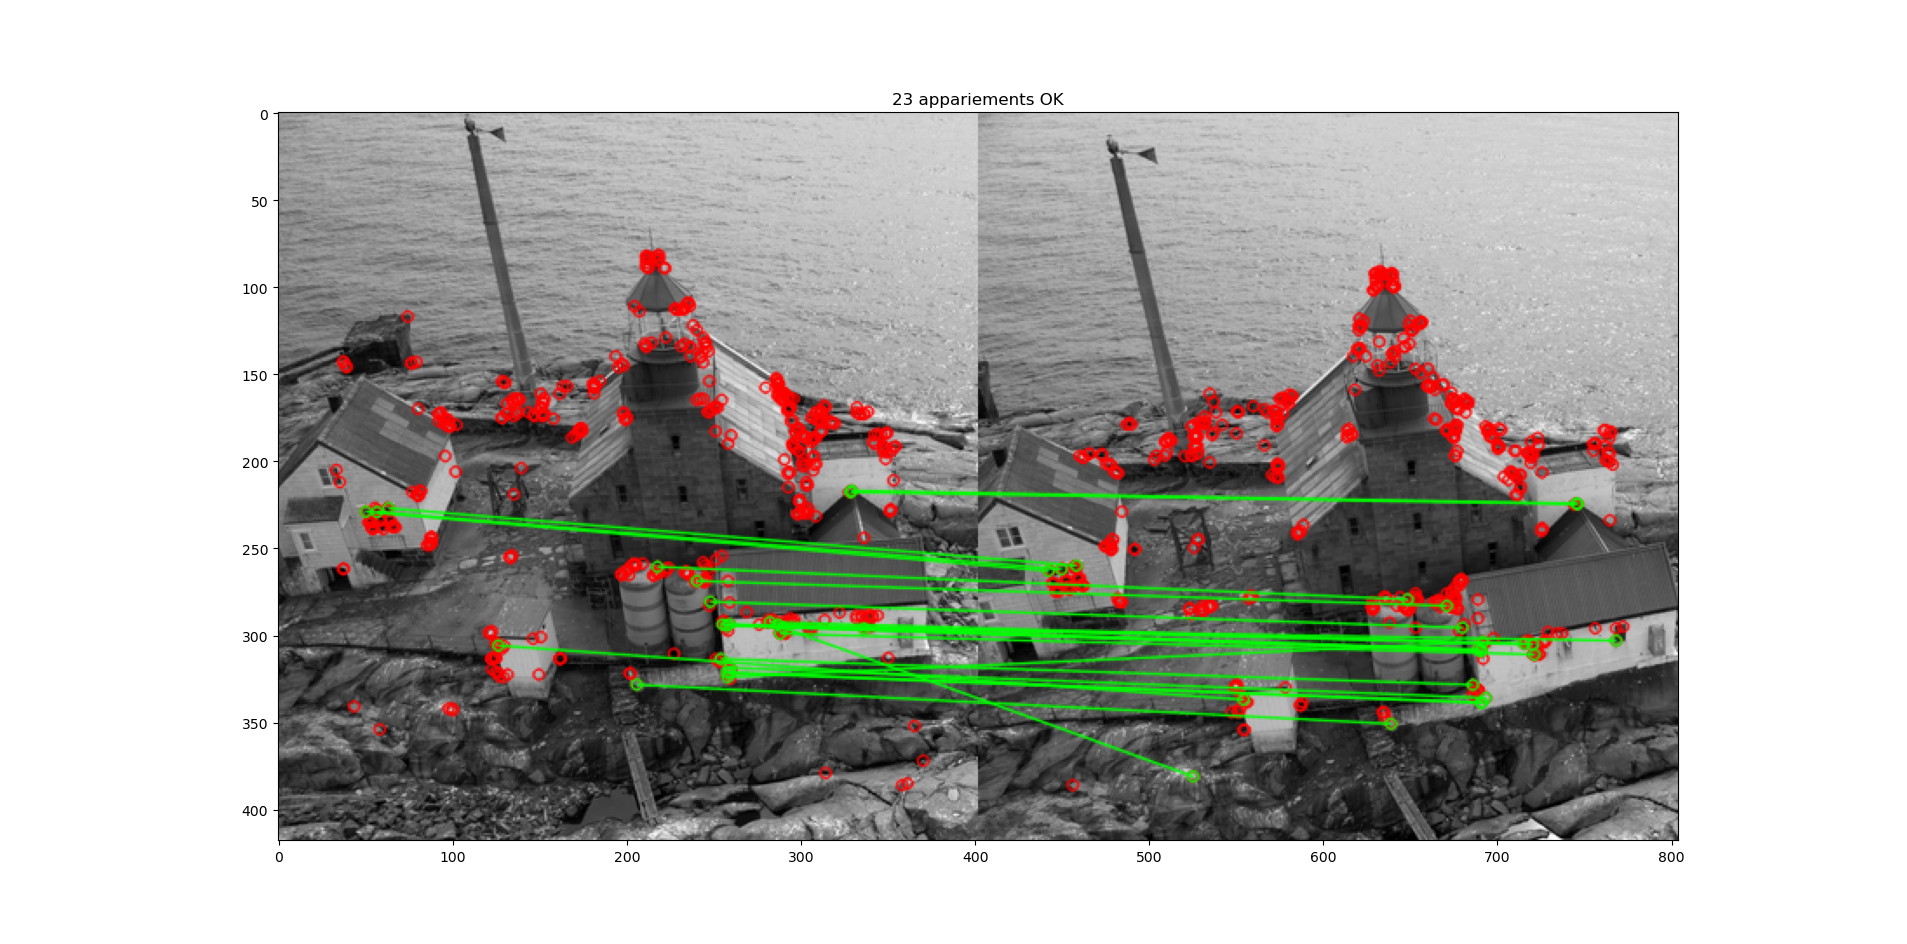
\includegraphics[trim= 50 40 50 40, clip = true, width=0.9\linewidth]{Images/ORB_FLANN.png}
		\caption{Résultats obtenus avec le méthode \textit{ORB} et \textit{FLANN}}
		\label{fig:orb_Flann}
	\end{figure}
	
	% ====================================================
	\begin{formal}
		\textbf{Q9 — Évaluation quantitative des correspondances}
	\end{formal}
	
	Une évaluation rigoureuse des performances d’appariement nécessite une référence géométrique connue.
	
	On applique une transformation affine ou projective connue à l’image initiale :
	
	$$
	M =
	\begin{bmatrix}
		s\cos\theta & -s\sin\theta & t_x \\
		s\sin\theta & s\cos\theta & t_y
	\end{bmatrix}
	$$
	
	Les points détectés dans l’image originale sont projetés théoriquement :
	
	$$
	p'_{th} = M p
	$$
	
	On compare ensuite ces positions théoriques aux positions effectivement détectées dans l’image transformée.
	
	L’erreur géométrique (erreur de reprojection) est définie par :
	
	$$
	e = \| p'_{detecté} - p'_{th} \|
	$$
	
	Les indicateurs statistiques pertinents incluent :
	- l’erreur moyenne,
	- la médiane,
	- le RMSE,
	- le pourcentage de correspondances dont l’erreur est inférieure à un seuil fixé (par exemple 3 pixels).
	
	Cette méthodologie permet une comparaison objective entre détecteurs et descripteurs, en quantifiant à la fois la précision et la robustesse des correspondances.
	
	\begin{figure}[H]
		\centering
		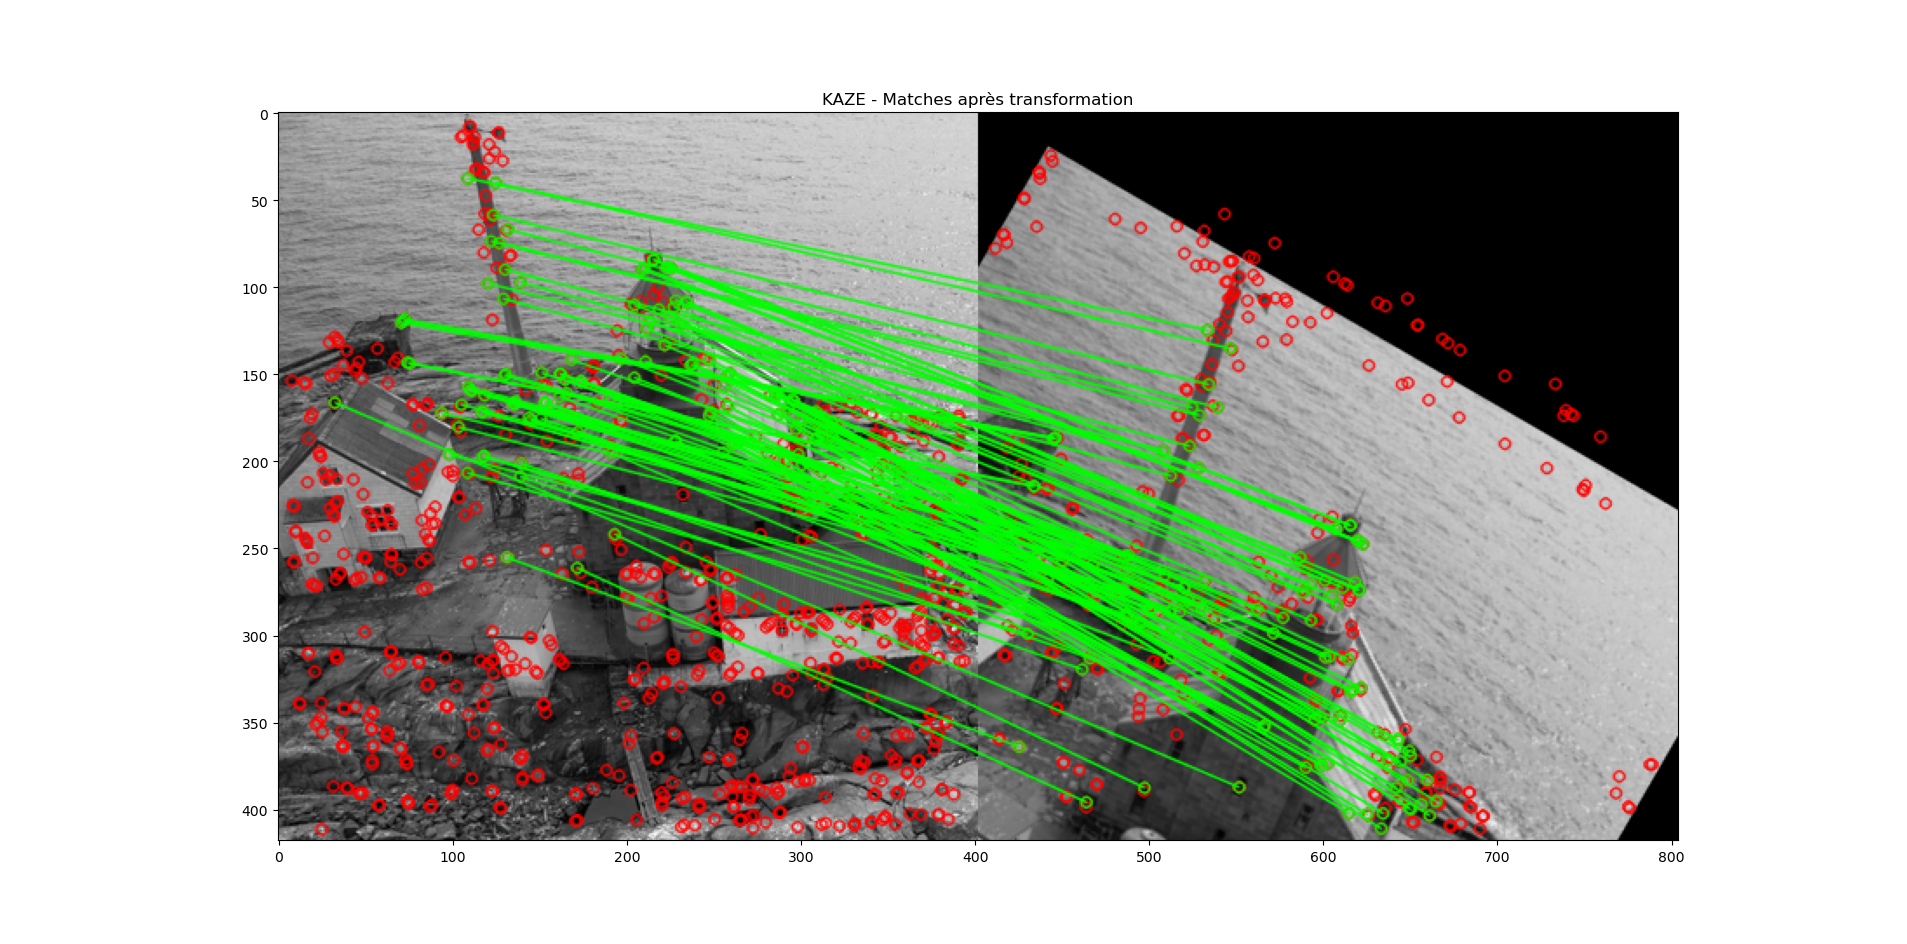
\includegraphics[trim= 50 40 50 40, clip = true, width=0.9\linewidth]{Images/Kaze_FLANN_Rotate.png}
		\caption{Résultats obtenus avec le méthode \textit{KAZE} et \textit{FLANN} et une rotation}
		\label{fig:kaze_FlannR}
	\end{figure}
	\begin{figure}[H]
		\centering
		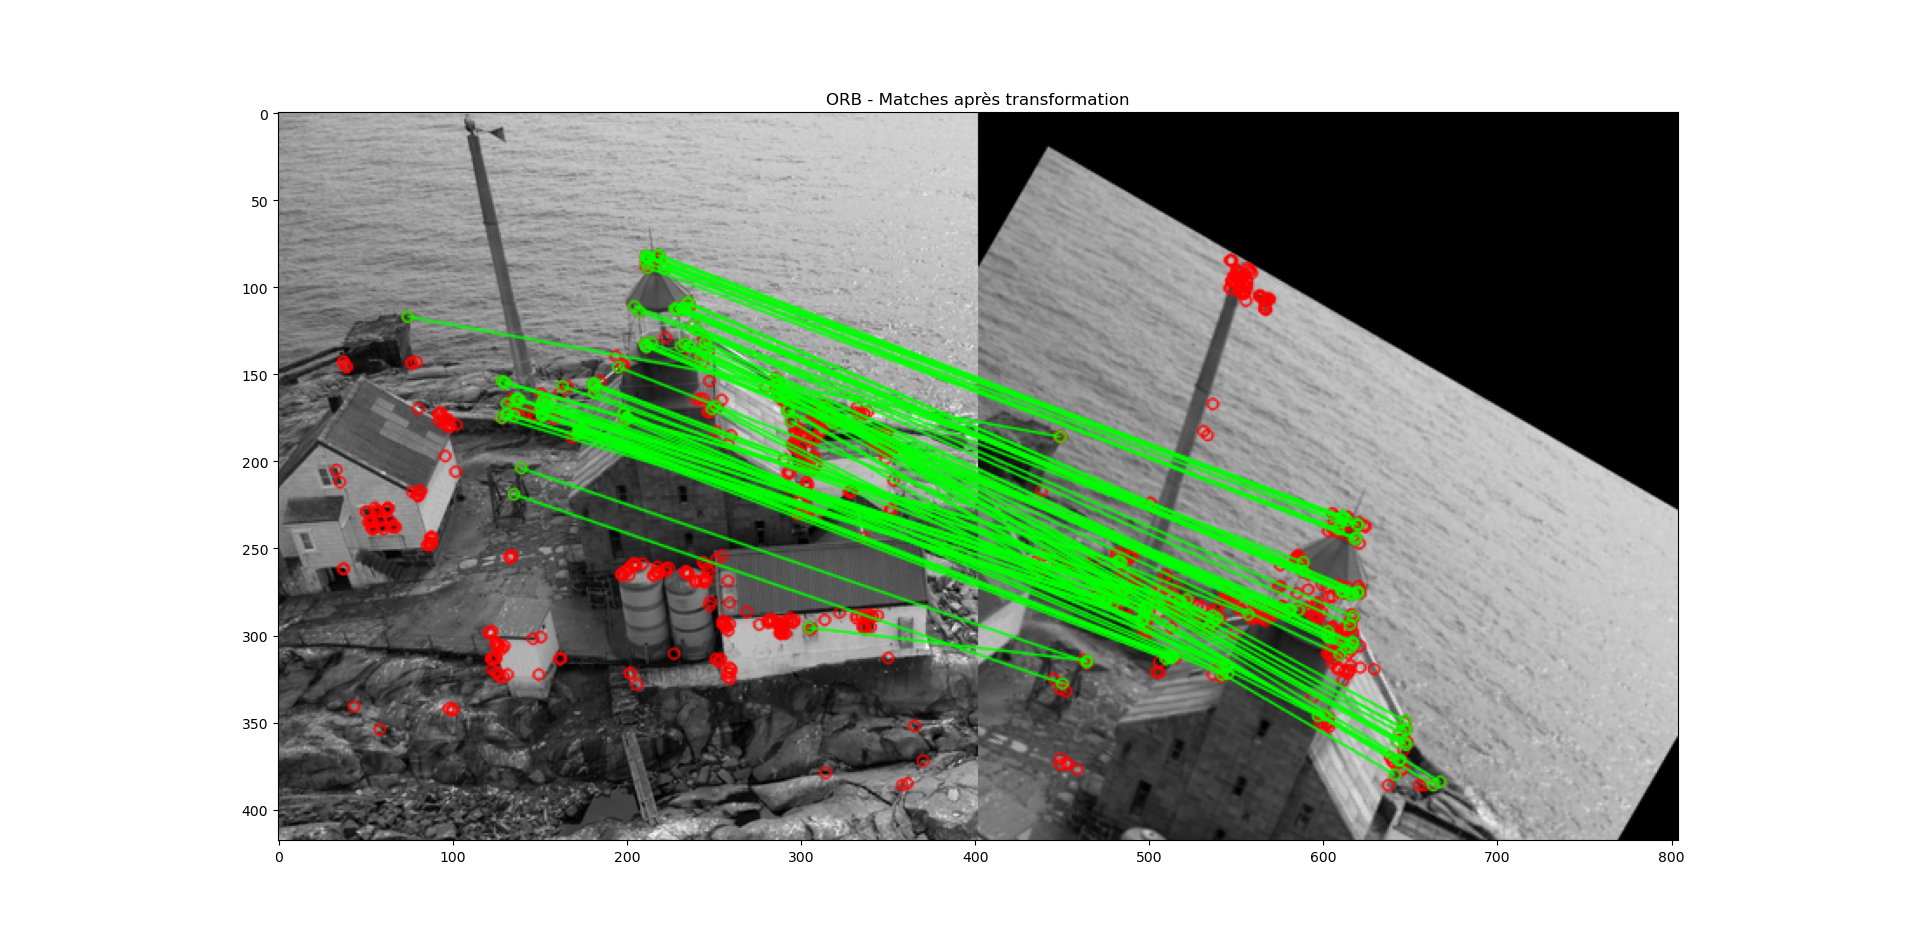
\includegraphics[trim= 50 40 50 40, clip = true, width=0.9\linewidth]{Images/ORB_FLANN_Rotate.png}
		\caption{Résultats obtenus avec le méthode \textit{ORB} et \textit{FLANN} et une rotation}
		\label{fig:orb_FlannR}
	\end{figure}
	
	\newpage
	% ====================================================
	% CONCLUSION
	% ====================================================
	
	\section*{Conclusion}
	
	Ce travail nous a permis d’étudier le lien entre les fondements mathématiques du traitement d’image et leur mise en oeuvre dans une algorithmique concrète. Les expériences réalisées montrent que les opérations telles que la convolution et le calcul du gradient constituent la base des méthodes de détection modernes.
	
	L’étude comparative de Harris, ORB et KAZE met en évidence différents compromis comme rapidité et efficacité pour les descripteurs binaires, robustesse accrue et modélisation plus fine pour les approches non linéaires. L’analyse des méthodes d’appariement confirme également l’importance des critères de sélection et des stratégies de validation géométrique.
	
	Ainsi, ce TP met en évidence que le choix d’un détecteur ou d’un descripteur dépend fortement du contexte applicatif, notamment des contraintes de précision, de robustesse et de complexité computationnelle.
	
	
	
	% ====================================================
	% RÉFÉRENCES
	% ====================================================
	\newpage
	\begin{thebibliography}{9}
		
		\bibitem{cours}
		Supports de cours MI204, ENSTA Paris.
		%\bibitem{ramberg}
		
		\bibitem{opencv}
		OpenCV Documentation, \url{https://docs.opencv.org/4.1.0/}
		
	\end{thebibliography}
	
\end{document}
